\documentclass[8pt]{beamer}

\usetheme{metropolis}

\usepackage[export]{adjustbox}
\usepackage{amsmath}
\usepackage{bbm}
\usepackage{emoji}
\usepackage{pgfplots}
\usepackage{hyperref}
\usepackage{listings}
\usepackage{tcolorbox}
\usepackage{xcolor}

\usepgfplotslibrary{groupplots}

\usetikzlibrary{arrows.meta}
\usetikzlibrary{calc}

\hypersetup{
    colorlinks=true,
    linkcolor=white,
    urlcolor=blue!80
}

\definecolor{uiored}{HTML}{DD0000}
\definecolor{uiolightred}{HTML}{FB6666}
\definecolor{uioredtone}{HTML}{FEE0E0}
\definecolor{uioblue}{HTML}{3E31D6}
\definecolor{uiolightblue}{HTML}{86A4F7}
\definecolor{uioblueone}{HTML}{E6ECFF}
\definecolor{uiogreen}{HTML}{2EC483}
\definecolor{uiolightgreen}{HTML}{6CE1AB}
\definecolor{uiogreentone}{HTML}{CEFFDF}
\definecolor{uioorange}{HTML}{FEA11B}
\definecolor{uiolightorange}{HTML}{FDCB87}
\definecolor{uioorangetone}{HTML}{FFE8D4}
\definecolor{uioyellow}{HTML}{FFFEA7}
\definecolor{uiogray}{HTML}{B2B3B7}

\colorlet{mainbackground}{uiored}

\setbeamercolor{frametitle}{bg=mainbackground, fg=white}
\setbeamercolor{title separator}{fg=mainbackground}
\setbeamercolor{progress bar in section page}{fg=white, bg=uiogray}

\def\logowidth{4cm}

\makeatletter
\setbeamertemplate{section page}
{
  \begingroup

    \vspace{4.3cm}
    {\usebeamercolor[fg]{section title}\usebeamerfont{section title}\insertsectionhead}\\[-1ex]
    {\centering\color{white}\rule{\linewidth}{1pt}\par} % the horizontal line

    \vspace*{3.1cm}
    \begin{center}
        
\includegraphics[width=\logowidth,valign=c]{data/uio_logo_full_white.png} % Adjust width and path to your logo as needed
    \end{center}

  \endgroup
}
\makeatother

\AtBeginSection{
  {
    \setbeamercolor{background canvas}{bg=uiored}
    \setbeamercolor{section title}{fg=white}
    \frame[plain,c,noframenumbering]{\sectionpage}
    \setbeamercolor{background canvas}{bg=black!2}
  }
}



\setbeamertemplate{footline}{
    \ifnum\insertframenumber=1
        % Title page, no footer
    \else
        \begin{tikzpicture}[remember picture,overlay]
            \fill[mainbackground] (current page.south west) rectangle ([yshift=0.45cm]current page.south east); % Draw filled rectangle

            % Logo
            \node[anchor=west, yshift=0.225cm] at (current page.south west) {
\includegraphics[height=1.2cm]{data/uio_logo_white.png}};

            % Title and subtitle
            \node[align=center, yshift=0.225cm] at (current page.south) {\textcolor{white}{\textbf{\inserttitle}}\\[0.05cm]\textcolor{white}{\insertsubtitle}};

            % Page number
            \node[anchor=east, yshift=0.225cm, xshift=-0.2cm, align=right] at (current page.south east) {\textcolor{white}{\insertframenumber/\inserttotalframenumber}};
        \end{tikzpicture}
    \fi
}

\lstdefinestyle{RStyle}{
    language=R,
    basicstyle=\ttfamily\fontsize{5}{6}\selectfont,
    keywordstyle=\color[RGB]{17, 115, 187},
    commentstyle=\color[RGB]{0, 128, 0},
    identifierstyle=\color[RGB]{0, 0, 0},
    stringstyle=\color[RGB]{205, 49, 49},
    numberstyle=\fontsize{5}{6}\selectfont\color[RGB]{128, 128, 128},
    numbers=left,
    numbersep=6pt,
    backgroundcolor=\color[RGB]{255, 255, 255},
    frame=single,
    rulecolor=\color[RGB]{0, 0, 0},
    showstringspaces=false,
    breaklines,
    xleftmargin=3pt,
    xrightmargin=3pt,
    framesep=3pt,
    aboveskip=-1.5pt,
    belowskip=-0.5pt,
    showlines=true
}

\lstdefinestyle{PythonStyle}{
    language=Python,
    basicstyle=\ttfamily\fontsize{5}{6}\selectfont,
    keywordstyle=\color[RGB]{26, 13, 171},
    commentstyle=\color[RGB]{0, 128, 0},
    identifierstyle=\color[RGB]{0, 0, 0},
    stringstyle=\color[RGB]{205, 49, 49},
    numberstyle=\fontsize{5}{6}\selectfont\color[RGB]{128, 128, 128},
    frame=tblr,
    backgroundcolor=\color[RGB]{245, 245, 245},
    rulecolor=\color[RGB]{192, 192, 192},
    showstringspaces=false,
    breaklines,
    xleftmargin=3pt,
    xrightmargin=3pt,
    framesep=3pt,
    aboveskip=-1.5pt,
    belowskip=-0.5pt,
    showlines=true,
}

\lstdefinestyle{ROutput}{
    language=R,
    basicstyle=\ttfamily\fontsize{5}{6}\selectfont,
    backgroundcolor=\color[RGB]{255, 255, 255},
    commentstyle=\color[HTML]{009900},
    stringstyle=\color[HTML]{0000FF},
    keywordstyle=\color[HTML]{000000},
    numberstyle=\tiny\color[HTML]{000000},
    breakatwhitespace=true,
    breaklines=true,
    frame=single,
    rulecolor=\color{black},
    showstringspaces=false,
    breaklines,
    xleftmargin=3pt,
    xrightmargin=3pt,
    framesep=3pt,
    aboveskip=-1.5pt,
    belowskip=-0.5pt,
    showlines=true
}

\lstdefinestyle{PythonOutput}{
    basicstyle=\fontsize{5}{6}\selectfont,
    backgroundcolor=\color[RGB]{255, 255, 255},
    rulecolor=\color[RGB]{192, 192, 192},
    frame=single,
    numbers=none,
    showstringspaces=false,
    breaklines=true,
    breakatwhitespace=true,
    showstringspaces=false,
    breaklines,
    xleftmargin=3pt,
    xrightmargin=3pt,
    framesep=3pt,
    aboveskip=-1.5pt,
    belowskip=-0.5pt,
    showlines=true,
    keywordstyle=\color[RGB]{255, 0, 0},
    morekeywords={AttributeError}
}

\title{PSY9511: Seminar 3}
\subtitle{Regularization and variable selection}
\author{Esten H. Leonardsen}
\date{07.09.23}

\begin{document}
	\begin{frame}
	 	\maketitle
	\end{frame}

    \begin{frame}{Outline}
        \centering
        \vfill
        \begin{enumerate}
            \item Assignment 1
            \item Assignment 2
            \item Regularization
            \begin{itemize}
                \item Variable selection
                \item Shrinkage (+ live coding \emoji{partying-face})
                \item Dimensionality reduction
            \end{itemize}
        \end{enumerate}
        \vfill
    \end{frame}

    \section{Assignment 1}

    \begin{frame}[t]{Assignment 1: Coding}
        \vspace{2cm}
        \begin{itemize}
            \item Create a vector of 100 standard normally distributed numbers and visualize them with a histogram.
            \item Show rows 5, 8, 9, and 10 of the Auto dataset.
            \item Show the last three columns of the Auto dataset.
            \item Show all cars with five cylinders in the Auto dataset.
        \end{itemize}

        \only<2>{
            \vspace{0.5cm}
            \url{http://localhost:8889/notebooks/notebooks\%2FAssignment\%201.ipynb}
        }
    \end{frame}

    \newcommand{\flexplot}[1]{
        \begin{tikzpicture}
            \begin{axis}[
                height=4cm,
                width=4cm,
                xmajorticks=false,
                ymajorticks=false,
                xmin=0,
                xmax=1,
                ymin=0,
                ymax=1
            ]
                \addplot[
                    only marks,
                    mark=*,
                    color=blue,
                    opacity=0.1
                ] table [
                    col sep=comma,
                    y=y,
                    x=X
                ] {data/flexibility.csv};

                \ifnum#1<7
                    \ifnum#1=1
                        \def\col{simple}
                    \fi
                    \ifnum#1=2
                        \def\col{medium}
                    \fi
                    \ifnum#1=3
                        \def\col{complex}
                    \fi
                    \ifnum#1=4
                        \def\col{k1}
                    \fi
                    \ifnum#1=5
                        \def\col{k30}
                    \fi
                    \ifnum#1=6
                        \def\col{k100}
                    \fi

                    \addplot[
                        very thick,
                        red
                    ] table [
                        col sep=comma,
                        y=\col,
                        x=X
                    ] {data/flexibility.csv};
                \fi
                \ifnum#1=7
                    \addplot[
                        very thick,
                        orange
                    ] table [
                        col sep=comma,
                        y=k100,
                        x=X
                    ] {data/flexibility.csv};
                \fi
                \ifnum#1=8
                    \addplot[
                        very thick,
                        red
                    ] table [
                        col sep=comma,
                        y=k30,
                        x=X
                    ] {data/flexibility.csv};
                    \addplot[
                        very thick,
                        orange
                    ] table [
                        col sep=comma,
                        y=approx,
                        x=X
                    ] {data/flexibility.csv};
                \fi
            \end{axis}
        \end{tikzpicture}
    }

    \newsavebox{\flexsimple}
    \sbox{\flexsimple}{\flexplot{1}}

    \newsavebox{\flexmedium}
    \sbox{\flexmedium}{\flexplot{2}}

    \newsavebox{\flexcomplex}
    \sbox{\flexcomplex}{\flexplot{3}}

    \newsavebox{\flexkone}
    \sbox{\flexkone}{\flexplot{4}}
    \newsavebox{\flexkthirty}
    \sbox{\flexkthirty}{\flexplot{5}}
    \newsavebox{\flexkall}
    \sbox{\flexkall}{\flexplot{6}}
    \newsavebox{\flexapproxall}
    \sbox{\flexapproxall}{\flexplot{7}}
    \newsavebox{\flexapprox}
    \sbox{\flexapprox}{\flexplot{8}}

    \newcommand{\biasvariance}[1]{
        \begin{tikzpicture}
            \begin{axis}[
                xmin=-1,
                xmax=1,
                ymin=-1,
                ymax=1,
                height=4cm,
                width=4cm,
                axis line style={draw=none},
                xmajorticks=false,
                ymajorticks=false
            ]
                \node[circle, minimum size=2.4cm, draw=black, fill=blue!60] at (axis cs: 0, 0) {};
                \node[circle, minimum size=1.9cm, draw=none, fill=white] at (axis cs: 0, 0) {};
                \node[circle, minimum size=1.4cm, draw=none, fill=blue!60] at (axis cs: 0, 0) {};
                \node[circle, minimum size=0.9cm, draw=none, fill=white] at (axis cs: 0, 0) {};
                \node[circle, minimum size=0.4cm, draw=none, fill=red] at (axis cs: 0, 0) {};

                \ifnum#1>1
                    \ifnum#1=2
                        \def\xcol{X1}
                        \def\ycol{y1}
                    \fi
                    \ifnum#1=3
                        \def\xcol{X2}
                        \def\ycol{y2}
                    \fi
                    \ifnum#1=4
                        \def\xcol{X3}
                        \def\ycol{y3}
                    \fi
                    \ifnum#1=5
                        \def\xcol{X4}
                        \def\ycol{y4}
                    \fi

                    \addplot[
                        only marks
                    ] table [
                        col sep=comma,
                        x=\xcol,
                        y=\ycol
                    ] {data/bias-variance.csv};
                \fi
            \end{axis}

        \end{tikzpicture}
    }

    \newsavebox{\dart}
    \sbox{\dart}{\biasvariance{1}}
    \newsavebox{\lowlow}
    \sbox{\lowlow}{\biasvariance{2}}
    \newsavebox{\lowhigh}
    \sbox{\lowhigh}{\biasvariance{3}}
    \newsavebox{\highlow}
    \sbox{\highlow}{\biasvariance{4}}
    \newsavebox{\highhigh}
    \sbox{\highhigh}{\biasvariance{5}}

    \begin{frame}{Assignment 2: Bias-variance trade-off}
        \only<1-9>{
            \begin{tikzpicture}
                \node[] at (-5.25, -3) {};
                \node[] at (5.25, 3) {};

                \only<2-6>{
                    \draw[-stealth] (-4, -1) -- (4, -1);
                }
                \only<2-3>{
                    \node[] at (0, -1.5) {Flexibility};
                }
                \only<3>{
                    \node[] at (-3, 1) {\usebox{\flexsimple}};
                    \node[] at (0, 1) {\usebox{\flexmedium}};
                    \node[] at (3, 1) {\usebox{\flexcomplex}};
                }
                \only<4-6>{
                    \node[] (kone) at (3, 1) {\usebox{\flexkone}};

                    \node[] at (0, -1.5) {Number of neighbours};
                    \draw[] (-3, -0.95) -- (-3, -1.05);
                    \node[anchor=north, inner sep=5pt] at (3, -1) {1};
                    \draw[] (3, -0.95) -- (3, -1.05);
                    \node[anchor=north, inner sep=5pt] at (-3, -1) {K};
                }
                \only<4>{
                    \node[] (kall) at (-3, 1) {\usebox{\flexkall}};
                }
                \only<4-5>{
                    \node[] (kthirty) at (0, 1) {\usebox{\flexkthirty}};
                }
                \only<5-9>{
                    \node[anchor=south,font=\tiny,orange, text depth=0] (formulak) at ($ (kall.south) - (0, 0.25) $) {$f(x)=0.39$};
                }
                \only<5-6>{
                    \node[] (kall) at (-3, 1) {\usebox{\flexapproxall}};
                }
                \only<6-9>{
                    \node[anchor=south,font=\tiny,orange, text depth=0] (formulaapprox) at ($ (kthirty.south) - (0, 0.25) $) {$f(x)=-3.57x^4+5.38x^3-1.22x^2+0.19x+0.03$};
                }
                \only<6>{
                    \node[] (kapprox) at (0, 1) {\usebox{\flexapprox}};
                }
                \only<8-9>{
                    \node[] (p11) at ($ (formulak.south) + (0.3, -0.3) $) {1};
                    \draw[-stealth] (p11.north) -- ($ (p11.north) + (0, 0.17) $);
                }\only<9>{
                    \node[] (p21) at ($ (formulaapprox.south) - (1.17, 0.3) $) {1};
                    \draw[-stealth] (p21.north) -- ($ (p21.north) + (0, 0.17) $);
                    \node[] (p22) at ($ (formulaapprox.south) - (0.32, 0.3) $) {2};
                    \draw[-stealth] (p22.north) -- ($ (p22.north) + (0, 0.17) $);
                    \node[] (p23) at ($ (formulaapprox.south) - (-0.44, 0.3) $) {3};
                    \draw[-stealth] (p23.north) -- ($ (p23.north) + (0, 0.17) $);
                    \node[] (p24) at ($ (formulaapprox.south) - (-1.26, 0.3) $) {4};
                    \draw[-stealth] (p24.north) -- ($ (p24.north) + (0, 0.17) $);
                    \node[] (p25) at ($ (formulaapprox.south) - (-1.95, 0.3) $) {5};
                    \draw[-stealth] (p25.north) -- ($ (p25.north) + (0, 0.17) $);
                }
            \end{tikzpicture}
        }
        \only<10>{
            Model flexibility: Denotes the complexity of the approximated function $\hat{y}=\hat{f}(x)$.
            \begin{itemize}
                \item Informally: Wigglyness of the line
                \item Formally: Number of parameters in the function (degrees of freedom)
            \end{itemize}
        }
        \only<11-15>{
            \begin{tikzpicture}
                \node[] at (-5.25, -3) {};
                \node[] at (5.25, 3) {};

                \only<11>{
                    \node[] at (-1.5, 1.5) {
                        \usebox{\dart}
                    };
                }
                \only<12-15>{
                    \node[] (lowlow) at (-1.5, 1.5) {
                        \usebox{\lowlow}
                    };
                    \node[anchor=south] at (lowlow.north) {Low variance};
                    \node[anchor=south, rotate=90] at (lowlow.west) {Low bias};
                }
                \only<13-15>{
                    \node[] (lowhigh) at (1.5, 1.5) {
                        \usebox{\lowhigh}
                    };
                    \node[anchor=south, text depth=0] at (lowhigh.north) {High variance};
                }
                \only<14-15>{
                    \node[] (highlow) at (-1.5, -1.5) {
                        \usebox{\highlow}
                    };
                    \node[anchor=south, text depth=0, rotate=90] at (highlow.west) {High bias};
                }
                \only<15>{
                    \node[] (highhigh) at (1.5, -1.5) {
                        \usebox{\highhigh}
                    };
                }

            \end{tikzpicture}
        }
    \end{frame}

    \section{Assignment 2}

    \begin{frame}{Assignment 2: Data splitting}
    \end{frame}

    \begin{frame}{Assignment 2: Random seeds}
    \end{frame}

    \begin{frame}{Assignment 2: Log-odds vs probability vs class}
    \end{frame}

    \begin{frame}{Assignment 2: Eye test}
    \end{frame}

    \section{Regularization}

    \begin{frame}{Regularization: Motivation}
        \centering
        \vfill
        $y \sim \beta_0 + \beta_1 * x_1 + \beta_2 * x_2 + \beta_3 * x_3$
        \vfill
    \end{frame}

    \begin{frame}{Regularization: Motivation}
        \centering
        \vfill
        \begin{tikzpicture}
            \node[draw=black, fill=white] {
                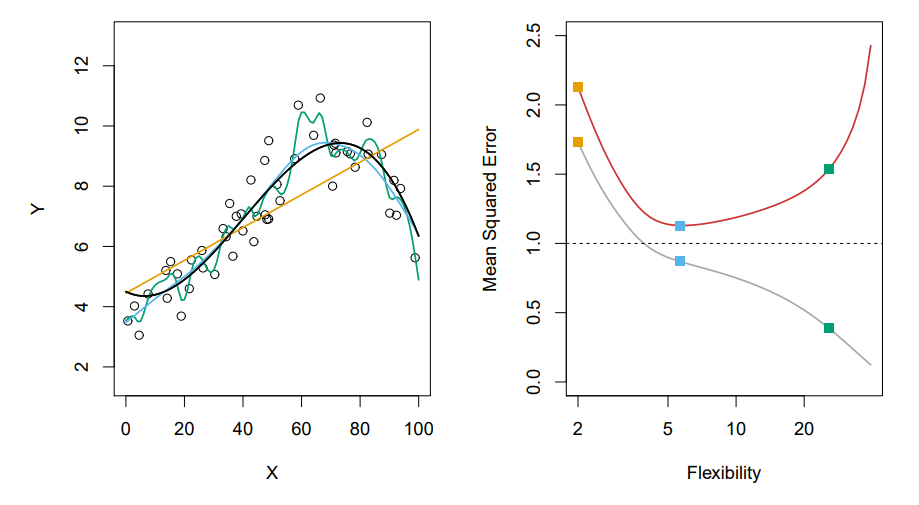
\includegraphics[width=8cm]{data/overfitting.png}
            };
        \end{tikzpicture}
        \vfill
    \end{frame}

    \begin{frame}{Regularization: Motivation}
        \centering
        \vfill
        $y \sim$\textcolor{red} {$ \beta_0 + \beta_1 * x_1 + \beta_2 * x_2 + \beta_3 * x_3$}
        \vfill
    \end{frame}

    \def\codewidth{0.9\textwidth}
    \begin{frame}[fragile]{Regularization: Out-of-sample testing}
        \begin{tikzpicture}
            \node[
                minimum width=\codewidth,
                text width=\codewidth,
                align=left,
                inner sep=0pt,
                anchor=north,
                label={[blue,
                        anchor=north east,
                        font=\ttfamily\fontsize{5}{6}\selectfont,
                        inner sep=0pt,
                        outer sep=0pt,
                        xshift=-3pt,
                        yshift=-3.5pt,
                        text depth=0
                        ]north west:In{[}1{]}:}
            ] (code) at (0, 0) {
                \begin{lstlisting}[style=PythonStyle]
import pandas as pd


df = pd.read_csv('/Users/esten/Downloads/Auto.csv')
train = df.iloc[:int(len(df) * 0.8)]
validation = df.iloc[int(len(df) * 0.8):]

print(f'Using {len(train)} samples for training')
print(f'Using {len(validation)} samples for validation')
                \end{lstlisting}
            };

            \node[
                minimum width=\codewidth,
                text width=\codewidth,
                align=left,
                inner sep=0pt,
                anchor=north,
                label={[red,
                        anchor=north east,
                        font=\ttfamily\fontsize{5}{6}\selectfont,
                        inner sep=0pt,
                        outer sep=0pt,
                        xshift=-3pt,
                        yshift=-3.5pt,
                        text depth=0
                        ]north west:Out{[}1{]}:}
            ] (output) at ($ (code.south) - (0, 0.2) $) {
                \begin{lstlisting}[style=PythonOutput]
Using 317 samples for training
Using 80 samples for validation
                \end{lstlisting}
            };
        \end{tikzpicture}
    \end{frame}

    \begin{frame}{Regularization: Methods}
        \begin{enumerate}
            \item Variable selection
            \begin{enumerate}
                \item[a.] Best subset selection
                \item[b.] Forward stepwise selection
                \item[c.] Backward stepwise selection
            \end{enumerate}
            \item Shrinkage
            \begin{enumerate}
                \item[a.] LASSO
                \item[b.] Ridge Regression
            \end{enumerate}
            \item Dimensionality reduction
            \begin{enumerate}
                \item[a.] Principal Component Regression
                \item[b.] Partial Least Squares
            \end{enumerate}
        \end{enumerate}
    \end{frame}

    \section{Variable selection}

    \begin{frame}{Variable selection: Motivation}
        \centering
        The number of predictors we are using in our model directly impacts model complexity.
    \end{frame}

    \begin{frame}[t]{Variable selection: Outline} % Problem definition
        \underline{Problem}\\
        We have a set of predictors $P=\{x_0, x_1, ...\}$ and a target variable $y$, and we want to find the subset $p \subseteq P$ that yields the best (linear) model for predicting $y$.\\
    \end{frame}

    \begin{frame}[t]{Variable selection: Outline} % Motivation
        \underline{Problem}\\
        We have a set of predictors $P=\{x_0, x_1, ...\}$ and a target variable $y$, and we want to find the subset $p \subseteq P$ that yields the best (linear) model for predicting $y$.\\
        \vspace{0.25cm}
        \underline{Motivation}\\
        \begin{enumerate}
            \item Reduce model complexity (overfitting)
            \item Simplify interpretation
        \end{enumerate}
    \end{frame}

    \def\codewidth{10cm}

    \begin{frame}[t]{Variable selection: Outline} % Variables
        \underline{Problem}\\
        We have a set of predictors $P=\{x_0, x_1, ...\}$ and a target variable $y$, and we want to find the subset $p \subseteq P$ that yields the best (linear) model for predicting $y$.\\
        \vspace{0.25cm}

        \centering
        \begin{tikzpicture}
            \begin{groupplot}[
                group style={
                    group size=3 by 2,
                    horizontal sep=0.5cm
                },
                ticklabel style = {font=\tiny},
                height=3.9cm,
                width=3.9cm
            ]
                \newcommand{\autoplot}[1]{
                    \nextgroupplot[
                        title=\scriptsize{####1},
                        every axis title/.style={at={(0.5,1.15)}}
                    ]
                        \addplot[
                            only marks,
                            mark=*,
                            color=blue,
                            opacity=0.25
                        ] table[
                            col sep=comma,
                            y=mpg,
                            x=####1
                        ] {data/Auto.csv};
                }
                \autoplot{cylinders}
                \autoplot{displacement}
                \autoplot{horsepower}
                \autoplot{weight}
                \autoplot{acceleration}
                \autoplot{year}
            \end{groupplot}

        \end{tikzpicture}
    \end{frame}

    \begin{frame}[t]{Variable selection: Best subset selection} % Implementation
        \underline{Problem}\\
        We have a set of predictors $P=\{x_0, x_1, ...\}$ and a target variable $y$, and we want to find the subset $p \subseteq P$ that yields the best (linear) model for predicting $y$.\\
        \vspace{0.25cm}
        \underline{Solution}\\
        Train models on all subsets $p$ and select the best one.
    \end{frame}

    \begin{frame}[t,fragile]{Variable selection: Best subset selection} % Implementation
        \underline{Problem}\\
        We have a set of predictors $P=\{x_0, x_1, ...\}$ and a target variable $y$, and we want to find the subset $p \subseteq P$ that yields the best (linear) model for predicting $y$.\\
        \vspace{0.25cm}
        \underline{Solution}\\
        \vspace{0.05cm}
        \centering
        \begin{tikzpicture}
            \node[
                minimum width=\codewidth,
                text width=\codewidth,
                align=left,
                inner sep=0pt,
                anchor=north,
                label={[blue,
                        anchor=north east,
                        font=\ttfamily\fontsize{4}{4}\selectfont,
                        inner sep=0pt,
                        outer sep=0pt,
                        xshift=-3pt,
                        yshift=-3.5pt,
                        text depth=0
                        ]north west:In{[}1{]}:}
            ] (code) at (0, 0) {
                \begin{lstlisting}[style=PythonStyle]
import numpy as np

from itertools import chain, combinations
from sklearn.linear_model import LinearRegression

subsets = list(chain.from_iterable(combinations(predictors, r) \
                                    for r in range(len(predictors)+1)))

best = {'mse': float('inf'), 'subset': None}

for subset in subsets:
    if len(subset) == 0:
        continue

    model = LinearRegression()
    model.fit(train[list(subset)], train[target])
    predictions = model.predict(validation[list(subset)])
    mse = np.mean((predictions - validation[target]) ** 2)

    if mse < best['mse']:
        best = {'mse': mse, 'subset': subset}

print(f'MSE: {best["mse"]:.2f}, predictors: {best["subset"]}')
                \end{lstlisting}
            };

            \node[
                minimum width=\codewidth,
                text width=\codewidth,
                align=left,
                inner sep=0pt,
                anchor=north,
                label={[red,
                        anchor=north east,
                        font=\ttfamily\fontsize{4}{4}\selectfont,
                        inner sep=0pt,
                        outer sep=0pt,
                        xshift=-3pt,
                        yshift=-3.5pt,
                        text depth=0
                        ]north west:Out{[}1{]}:}
            ] (output) at ($ (code.south) - (0, 0.1) $) {
                \begin{lstlisting}[style=PythonOutput]
MSE: 29.68, predictors: ('cylinders', 'displacement', 'horsepower', 'weight', 'year')                \end{lstlisting}
            };

        \end{tikzpicture}

    \end{frame}

     \begin{frame}[t]{Variable selection: Best subset selection} % Summary
        \underline{Problem}\\
        We have a set of predictors $P=\{x_0, x_1, ...\}$ and a target variable $y$, and we want to find the subset $p \subseteq P$ that yields the best (linear) model for predicting $y$.\\
        \vspace{0.25cm}
        \underline{Solution}\\
        Train models on all subsets $p$ and select the best one.\\
        \vspace{0.25cm}
        \underline{\textcolor{green}{+} Positives}\\
        Guaranteed to find the optimal solution.\\
        Simple implementation\\
        \vspace{0.25cm}
        \underline{\textcolor{red}{-} Drawbacks}\\
        Need to train many ($2^{|P|}$) models.
     \end{frame}

     \begin{frame}[t]{Variable selection: Best subset selection} % Number of models
        \centering
        \vfill
        \begin{tikzpicture}
            \begin{axis}[
                smooth,
                xmin=0,
                xmax=10,
                ymin=0,
                ymax=1200,
                xlabel={Number of predictors},
                ylabel={Number of models},
            ]
                \addplot[mark=*] coordinates {
                    (1, 2^1)
                    (2, 2^2)
                    (3, 2^3)
                    (4, 2^4)
                    (5, 2^5)
                    (6, 2^6)
                    (7, 2^7)
                    (8, 2^8)
                    (9, 2^9)
                    (10, 2^10)
                };
                \node[anchor=south] at (axis cs: 6, 2^6) {64};
            \end{axis}
        \end{tikzpicture}
        \vfill
     \end{frame}

     \begin{frame}[t]{Variable selection: Forward stepwise selection} % Intro
        \underline{Problem}\\
        We have a set of predictors $P=\{x_0, x_1, ...\}$ and a target variable $y$, and we want to find the subset $p \subseteq P$ that yields the best (linear) model for predicting $y$.\\
        \vspace{0.25cm}
        \underline{Solution}\\
        Start with no predictors. Iteratively add the predictor that yields the best model until all are included.\\
    \end{frame}

    \begin{frame}[t]{Variable selection: Forward stepwise selection} % Empty model
        \underline{Problem}\\
        We have a set of predictors $P=\{x_0, x_1, ...\}$ and a target variable $y$, and we want to find the subset $p \subseteq P$ that yields the best (linear) model for predicting $y$.\\
        \vspace{0.25cm}
        \underline{Solution}\\
        Start with no predictors. Iteratively add the predictor that yields the best model until all are included.\\
        \vspace{0.25cm}
        \centering

        \def\nodefont{\fontsize{4}{4}\linespread{0.85}\selectfont}
        \def\hsep{1.6}
        \def\vsep{0.75}
        \begin{tikzpicture}
            \node[draw=black, align=center, font=\nodefont] (n00) at (0, 0 * \vsep) {
                $y \sim \mathbbm{1}$\\
                $mse=146.47$
            };

            \node[] at (6.5 * \hsep, 3.3 * \vsep) {};
            \node[] at (-0.32 * \hsep, -3.3 * \vsep) {};
        \end{tikzpicture}
    \end{frame}

    \begin{frame}[t]{Variable selection: Forward stepwise selection} % n-5
        \underline{Problem}\\
        We have a set of predictors $P=\{x_0, x_1, ...\}$ and a target variable $y$, and we want to find the subset $p \subseteq P$ that yields the best (linear) model for predicting $y$.\\
        \vspace{0.25cm}
        \underline{Solution}\\
        Start with no predictors. Iteratively add the predictor that yields the best model until all are included.\\
        \vspace{0.25cm}
        \centering

        \def\nodefont{\fontsize{4}{4}\linespread{0.85}\selectfont}
        \def\hsep{1.6}
        \def\vsep{0.75}
        \begin{tikzpicture}
            \node[draw=black, align=center, font=\nodefont] (n00) at (0, 0 * \vsep) {
                $y \sim \mathbbm{1}$\\
                $mse=146.47$
            };

            \node[draw=black, align=center, font=\nodefont, color=black] (n11) at (\hsep, 2.5 * \vsep) {
                $y \sim cylinders$\\
                $67.96$
            };
            \node[draw=black, align=center, font=\nodefont, color=black] (n12) at (\hsep, 1.5 * \vsep) {
                $y \sim year$\\
                $61.56$
            };
            \node[draw=black, align=center, font=\nodefont, color=black] (n13) at (\hsep, 0.5 * \vsep) {
                $y \sim acceleration$\\
                $119.72$
            };
            \node[draw=black, align=center, font=\nodefont] (n14) at (\hsep, -0.5 * \vsep) {
                $y \sim weight$\\
                $61.18$
            };
            \node[draw=black, align=center, font=\nodefont, color=black] (n15) at (\hsep, -1.5 * \vsep) {
                $y \sim horsepower$\\
                $65.75$
            };
            \node[draw=black, align=center, font=\nodefont, color=black] (n16) at (\hsep, -2.5 * \vsep) {
                $y \sim displacement$\\
                $63.84$
            };


            \draw[black] (n00.east) -- (n11.west);
            \draw[black] (n00.east) -- (n12.west);
            \draw[black] (n00.east) -- (n13.west);
            \draw[black] (n00.east) -- (n14.west);
            \draw[black] (n00.east) -- (n15.west);
            \draw[black] (n00.east) -- (n16.west);

            \node[] at (6.5 * \hsep, 3.3 * \vsep) {};
            \node[] at (-0.32 * \hsep, -3.3 * \vsep) {};

        \end{tikzpicture}
    \end{frame}

    \begin{frame}[t]{Variable selection: Forward stepwise selection} % n-4
        \underline{Problem}\\
        We have a set of predictors $P=\{x_0, x_1, ...\}$ and a target variable $y$, and we want to find the subset $p \subseteq P$ that yields the best (linear) model for predicting $y$.\\
        \vspace{0.25cm}
        \underline{Solution}\\
        Start with no predictors. Iteratively add the predictor that yields the best model until all are included.\\
        \vspace{0.25cm}
        \centering

        \def\nodefont{\fontsize{4}{4}\linespread{0.85}\selectfont}
        \def\hsep{1.6}
        \def\vsep{0.75}
        \begin{tikzpicture}
            \node[draw=black, align=center, font=\nodefont] (n00) at (0, 0 * \vsep) {
                $y \sim \mathbbm{1}$\\
                $mse=146.47$
            };

            \node[draw=gray!25, align=center, font=\nodefont, color=gray!25] (n11) at (\hsep, 2.5 * \vsep) {
                $y \sim cylinders$\\
                $67.96$
            };
            \node[draw=gray!25, align=center, font=\nodefont, color=gray!25] (n12) at (\hsep, 1.5 * \vsep) {
                $y \sim year$\\
                $61.56$
            };
            \node[draw=gray!25, align=center, font=\nodefont, color=gray!25] (n13) at (\hsep, 0.5 * \vsep) {
                $y \sim acceleration$\\
                $119.72$
            };
            \node[draw=black, align=center, font=\nodefont] (n14) at (\hsep, -0.5 * \vsep) {
                $y \sim weight$\\
                $61.18$
            };
            \node[draw=gray!25, align=center, font=\nodefont, color=gray!25] (n15) at (\hsep, -1.5 * \vsep) {
                $y \sim horsepower$\\
                $65.75$
            };
            \node[draw=gray!25, align=center, font=\nodefont, color=gray!25] (n16) at (\hsep, -2.5 * \vsep) {
                $y \sim displacement$\\
                $63.84$
            };

            \node[draw=black, align=center, font=\nodefont, color=black] (n21) at (2 * \hsep, 2.5 * \vsep) {
                $\begin{aligned}
                    y\sim&weight +\\[-0.8em]
                    &cylinders
                \end{aligned}$\\
                $60.02$
            };
            \node[draw=black, align=center, font=\nodefont] (n22) at (2 * \hsep, 1.25 * \vsep) {
                $\begin{aligned}
                    y\sim&weight +\\[-0.8em]
                    &year
                \end{aligned}$\\
                $29.84$
            };
            \node[draw=black, align=center, font=\nodefont, color=black] (n23) at (2 * \hsep, 0 * \vsep) {
                $\begin{aligned}
                    y\sim&weight +\\[-0.8em]
                    &acceleration
                \end{aligned}$\\
                $60.01$
            };
            \node[draw=black, align=center, font=\nodefont, color=black] (n24) at (2 * \hsep, -1.25 * \vsep) {
                $\begin{aligned}
                    y\sim&weight +\\[-0.8em]
                    &horsepower
                \end{aligned}$\\
                $58.59$
            };
            \node[draw=black, align=center, font=\nodefont, color=black] (n25) at (2 * \hsep, -2.5 * \vsep) {
                $\begin{aligned}
                    y\sim&weight +\\[-0.8em]
                    &displacement
                \end{aligned}$\\
                $59.91$
            };

            \draw[gray!25] (n00.east) -- (n11.west);
            \draw[gray!25] (n00.east) -- (n12.west);
            \draw[gray!25] (n00.east) -- (n13.west);
            \draw[black] (n00.east) -- (n14.west);
            \draw[gray!25] (n00.east) -- (n15.west);
            \draw[gray!25] (n00.east) -- (n16.west);

            \draw[black] (n14.east) -- (n21.west);
            \draw[black] (n14.east) -- (n22.west);
            \draw[black] (n14.east) -- (n23.west);
            \draw[black] (n14.east) -- (n24.west);
            \draw[black] (n14.east) -- (n25.west);

            \node[] at (6.5 * \hsep, 3.3 * \vsep) {};
            \node[] at (-0.32 * \hsep, -3.3 * \vsep) {};

        \end{tikzpicture}
    \end{frame}

    \begin{frame}[t]{Variable selection: Forward stepwise selection} % n-3
        \underline{Problem}\\
        We have a set of predictors $P=\{x_0, x_1, ...\}$ and a target variable $y$, and we want to find the subset $p \subseteq P$ that yields the best (linear) model for predicting $y$.\\
        \vspace{0.25cm}
        \underline{Solution}\\
        Start with no predictors. Iteratively add the predictor that yields the best model until all are included.\\
        \vspace{0.25cm}
        \centering

        \def\nodefont{\fontsize{4}{4}\linespread{0.85}\selectfont}
        \def\hsep{1.6}
        \def\vsep{0.75}
        \begin{tikzpicture}
            \node[draw=black, align=center, font=\nodefont] (n00) at (0, 0 * \vsep) {
                $y \sim \mathbbm{1}$\\
                $mse=146.47$
            };

            \node[draw=gray!25, align=center, font=\nodefont, color=gray!25] (n11) at (\hsep, 2.5 * \vsep) {
                $y \sim cylinders$\\
                $67.96$
            };
            \node[draw=gray!25, align=center, font=\nodefont, color=gray!25] (n12) at (\hsep, 1.5 * \vsep) {
                $y \sim year$\\
                $61.56$
            };
            \node[draw=gray!25, align=center, font=\nodefont, color=gray!25] (n13) at (\hsep, 0.5 * \vsep) {
                $y \sim acceleration$\\
                $119.72$
            };
            \node[draw=black, align=center, font=\nodefont] (n14) at (\hsep, -0.5 * \vsep) {
                $y \sim weight$\\
                $61.18$
            };
            \node[draw=gray!25, align=center, font=\nodefont, color=gray!25] (n15) at (\hsep, -1.5 * \vsep) {
                $y \sim horsepower$\\
                $65.75$
            };
            \node[draw=gray!25, align=center, font=\nodefont, color=gray!25] (n16) at (\hsep, -2.5 * \vsep) {
                $y \sim displacement$\\
                $63.84$
            };

            \node[draw=gray!25, align=center, font=\nodefont, color=gray!25] (n21) at (2 * \hsep, 2.5 * \vsep) {
                $\begin{aligned}
                    y\sim&weight +\\[-0.8em]
                    &cylinders
                \end{aligned}$\\
                $60.02$
            };
            \node[draw=black, align=center, font=\nodefont] (n22) at (2 * \hsep, 1.25 * \vsep) {
                $\begin{aligned}
                    y\sim&weight +\\[-0.8em]
                    &year
                \end{aligned}$\\
                $29.84$
            };
            \node[draw=gray!25, align=center, font=\nodefont, color=gray!25] (n23) at (2 * \hsep, 0 * \vsep) {
                $\begin{aligned}
                    y\sim&weight +\\[-0.8em]
                    &acceleration
                \end{aligned}$\\
                $60.01$
            };
            \node[draw=gray!25, align=center, font=\nodefont, color=gray!25] (n24) at (2 * \hsep, -1.25 * \vsep) {
                $\begin{aligned}
                    y\sim&weight +\\[-0.8em]
                    &horsepower
                \end{aligned}$\\
                $58.59$
            };
            \node[draw=gray!25, align=center, font=\nodefont, color=gray!25] (n25) at (2 * \hsep, -2.5 * \vsep) {
                $\begin{aligned}
                    y\sim&weight +\\[-0.8em]
                    &displacement
                \end{aligned}$\\
                $59.91$
            };

            \node[draw=black, align=center, font=\nodefont, color=black] (n31) at (3 * \hsep, 2.25 * \vsep) {
                $\begin{aligned}
                    y\sim&weight +\\[-0.8em]
                    &year +\\[-0.8em]
                    &cylinders
                \end{aligned}$\\
                $29.91$
            };
            \node[draw=black, align=center, font=\nodefont, color=black] (n32) at (3 * \hsep, 0.75 * \vsep) {
                $\begin{aligned}
                    y\sim&weight +\\[-0.8em]
                    &year +\\[-0.8em]
                    &acceleration
                \end{aligned}$\\
                $29.99$
            };
            \node[draw=black, align=center, font=\nodefont] (n33) at (3 * \hsep, -0.75 * \vsep) {
                $\begin{aligned}
                    y\sim&weight +\\[-0.8em]
                    &year +\\[-0.8em]
                    &horsepower
                \end{aligned}$\\
                $29.85$
            };
            \node[draw=black, align=center, font=\nodefont, color=black] (n34) at (3 * \hsep, -2.25 * \vsep) {
                $\begin{aligned}
                    y\sim&weight +\\[-0.8em]
                    &year +\\[-0.8em]
                    &displacement
                \end{aligned}$\\
                $29.96$
            };

            \draw[gray!25] (n00.east) -- (n11.west);
            \draw[gray!25] (n00.east) -- (n12.west);
            \draw[gray!25] (n00.east) -- (n13.west);
            \draw[black] (n00.east) -- (n14.west);
            \draw[gray!25] (n00.east) -- (n15.west);
            \draw[gray!25] (n00.east) -- (n16.west);

            \draw[gray!25] (n14.east) -- (n21.west);
            \draw[black] (n14.east) -- (n22.west);
            \draw[gray!25] (n14.east) -- (n23.west);
            \draw[gray!25] (n14.east) -- (n24.west);
            \draw[gray!25] (n14.east) -- (n25.west);

            \draw[black] (n22.east) -- (n31.west);
            \draw[black] (n22.east) -- (n32.west);
            \draw[black] (n22.east) -- (n33.west);
            \draw[black] (n22.east) -- (n34.west);

            \node[] at (6.5 * \hsep, 3.3 * \vsep) {};
            \node[] at (-0.32 * \hsep, -3.3 * \vsep) {};

        \end{tikzpicture}
    \end{frame}

    \begin{frame}[t]{Variable selection: Forward stepwise selection} % n-2
        \underline{Problem}\\
        We have a set of predictors $P=\{x_0, x_1, ...\}$ and a target variable $y$, and we want to find the subset $p \subseteq P$ that yields the best (linear) model for predicting $y$.\\
        \vspace{0.25cm}
        \underline{Solution}\\
        Start with no predictors. Iteratively add the predictor that yields the best model until all are included.\\
        \vspace{0.25cm}
        \centering

        \def\nodefont{\fontsize{4}{4}\linespread{0.85}\selectfont}
        \def\hsep{1.6}
        \def\vsep{0.75}
        \begin{tikzpicture}
            \node[draw=black, align=center, font=\nodefont] (n00) at (0, 0 * \vsep) {
                $y \sim \mathbbm{1}$\\
                $mse=146.47$
            };

            \node[draw=gray!25, align=center, font=\nodefont, color=gray!25] (n11) at (\hsep, 2.5 * \vsep) {
                $y \sim cylinders$\\
                $67.96$
            };
            \node[draw=gray!25, align=center, font=\nodefont, color=gray!25] (n12) at (\hsep, 1.5 * \vsep) {
                $y \sim year$\\
                $61.56$
            };
            \node[draw=gray!25, align=center, font=\nodefont, color=gray!25] (n13) at (\hsep, 0.5 * \vsep) {
                $y \sim acceleration$\\
                $119.72$
            };
            \node[draw=black, align=center, font=\nodefont] (n14) at (\hsep, -0.5 * \vsep) {
                $y \sim weight$\\
                $61.18$
            };
            \node[draw=gray!25, align=center, font=\nodefont, color=gray!25] (n15) at (\hsep, -1.5 * \vsep) {
                $y \sim horsepower$\\
                $65.75$
            };
            \node[draw=gray!25, align=center, font=\nodefont, color=gray!25] (n16) at (\hsep, -2.5 * \vsep) {
                $y \sim displacement$\\
                $63.84$
            };

            \node[draw=gray!25, align=center, font=\nodefont, color=gray!25] (n21) at (2 * \hsep, 2.5 * \vsep) {
                $\begin{aligned}
                    y\sim&weight +\\[-0.8em]
                    &cylinders
                \end{aligned}$\\
                $60.02$
            };
            \node[draw=black, align=center, font=\nodefont] (n22) at (2 * \hsep, 1.25 * \vsep) {
                $\begin{aligned}
                    y\sim&weight +\\[-0.8em]
                    &year
                \end{aligned}$\\
                $29.84$
            };
            \node[draw=gray!25, align=center, font=\nodefont, color=gray!25] (n23) at (2 * \hsep, 0 * \vsep) {
                $\begin{aligned}
                    y\sim&weight +\\[-0.8em]
                    &acceleration
                \end{aligned}$\\
                $60.01$
            };
            \node[draw=gray!25, align=center, font=\nodefont, color=gray!25] (n24) at (2 * \hsep, -1.25 * \vsep) {
                $\begin{aligned}
                    y\sim&weight +\\[-0.8em]
                    &horsepower
                \end{aligned}$\\
                $58.59$
            };
            \node[draw=gray!25, align=center, font=\nodefont, color=gray!25] (n25) at (2 * \hsep, -2.5 * \vsep) {
                $\begin{aligned}
                    y\sim&weight +\\[-0.8em]
                    &displacement
                \end{aligned}$\\
                $59.91$
            };

            \node[draw=gray!25, align=center, font=\nodefont, color=gray!25] (n31) at (3 * \hsep, 2.25 * \vsep) {
                $\begin{aligned}
                    y\sim&weight +\\[-0.8em]
                    &year +\\[-0.8em]
                    &cylinders
                \end{aligned}$\\
                $29.91$
            };
            \node[draw=gray!25, align=center, font=\nodefont, color=gray!25] (n32) at (3 * \hsep, 0.75 * \vsep) {
                $\begin{aligned}
                    y\sim&weight +\\[-0.8em]
                    &year +\\[-0.8em]
                    &acceleration
                \end{aligned}$\\
                $29.99$
            };
            \node[draw=black, align=center, font=\nodefont] (n33) at (3 * \hsep, -0.75 * \vsep) {
                $\begin{aligned}
                    y\sim&weight +\\[-0.8em]
                    &year +\\[-0.8em]
                    &horsepower
                \end{aligned}$\\
                $29.85$
            };
            \node[draw=gray!25, align=center, font=\nodefont, color=gray!25] (n34) at (3 * \hsep, -2.25 * \vsep) {
                $\begin{aligned}
                    y\sim&weight +\\[-0.8em]
                    &year +\\[-0.8em]
                    &displacement
                \end{aligned}$\\
                $29.96$
            };

            \node[draw=black, align=center, font=\nodefont, color=black] (n41) at (4 * \hsep, 1.75 * \vsep) {
                $\begin{aligned}
                    y\sim&weight +\\[-0.8em]
                    &year +\\[-0.8em]
                    &horsepower +\\[-0.8em]
                    &cylinders
                \end{aligned}$\\
                $29.87$
            };
            \node[draw=black, align=center, font=\nodefont, color=black] (n42) at (4 * \hsep, 0 * \vsep) {
                $\begin{aligned}
                    y\sim&weight +\\[-0.8em]
                    &year +\\[-0.8em]
                    &horsepower +\\[-0.8em]
                    &acceleration
                \end{aligned}$\\
                $30.29$
            };
            \node[draw=black, align=center, font=\nodefont, color=black] (n43) at (4 * \hsep, -1.75 * \vsep) {
                $\begin{aligned}
                    y\sim&weight +\\[-0.8em]
                    &year +\\[-0.8em]
                    &horsepower +\\[-0.8em]
                    &displacement
                \end{aligned}$\\
                $29.95$
            };


            \draw[gray!25] (n00.east) -- (n11.west);
            \draw[gray!25] (n00.east) -- (n12.west);
            \draw[gray!25] (n00.east) -- (n13.west);
            \draw[black] (n00.east) -- (n14.west);
            \draw[gray!25] (n00.east) -- (n15.west);
            \draw[gray!25] (n00.east) -- (n16.west);

            \draw[gray!25] (n14.east) -- (n21.west);
            \draw[black] (n14.east) -- (n22.west);
            \draw[gray!25] (n14.east) -- (n23.west);
            \draw[gray!25] (n14.east) -- (n24.west);
            \draw[gray!25] (n14.east) -- (n25.west);

            \draw[gray!25] (n22.east) -- (n31.west);
            \draw[gray!25] (n22.east) -- (n32.west);
            \draw[black] (n22.east) -- (n33.west);
            \draw[gray!25] (n22.east) -- (n34.west);

            \draw[black] (n33.east) -- (n41.west);
            \draw[black] (n33.east) -- (n42.west);
            \draw[black] (n33.east) -- (n43.west);

            \node[] at (6.5 * \hsep, 3.3 * \vsep) {};
            \node[] at (-0.32 * \hsep, -3.3 * \vsep) {};

        \end{tikzpicture}
    \end{frame}

    \begin{frame}[t]{Variable selection: Forward stepwise selection} % n-1
        \underline{Problem}\\
        We have a set of predictors $P=\{x_0, x_1, ...\}$ and a target variable $y$, and we want to find the subset $p \subseteq P$ that yields the best (linear) model for predicting $y$.\\
        \vspace{0.25cm}
        \underline{Solution}\\
        Start with no predictors. Iteratively add the predictor that yields the best model until all are included.\\
        \vspace{0.25cm}
        \centering

        \def\nodefont{\fontsize{4}{4}\linespread{0.85}\selectfont}
        \def\hsep{1.6}
        \def\vsep{0.75}
        \begin{tikzpicture}
            \node[draw=black, align=center, font=\nodefont] (n00) at (0, 0 * \vsep) {
                $y \sim \mathbbm{1}$\\
                $mse=146.47$
            };

            \node[draw=gray!25, align=center, font=\nodefont, color=gray!25] (n11) at (\hsep, 2.5 * \vsep) {
                $y \sim cylinders$\\
                $67.96$
            };
            \node[draw=gray!25, align=center, font=\nodefont, color=gray!25] (n12) at (\hsep, 1.5 * \vsep) {
                $y \sim year$\\
                $61.56$
            };
            \node[draw=gray!25, align=center, font=\nodefont, color=gray!25] (n13) at (\hsep, 0.5 * \vsep) {
                $y \sim acceleration$\\
                $119.72$
            };
            \node[draw=black, align=center, font=\nodefont] (n14) at (\hsep, -0.5 * \vsep) {
                $y \sim weight$\\
                $61.18$
            };
            \node[draw=gray!25, align=center, font=\nodefont, color=gray!25] (n15) at (\hsep, -1.5 * \vsep) {
                $y \sim horsepower$\\
                $65.75$
            };
            \node[draw=gray!25, align=center, font=\nodefont, color=gray!25] (n16) at (\hsep, -2.5 * \vsep) {
                $y \sim displacement$\\
                $63.84$
            };

            \node[draw=gray!25, align=center, font=\nodefont, color=gray!25] (n21) at (2 * \hsep, 2.5 * \vsep) {
                $\begin{aligned}
                    y\sim&weight +\\[-0.8em]
                    &cylinders
                \end{aligned}$\\
                $60.02$
            };
            \node[draw=black, align=center, font=\nodefont] (n22) at (2 * \hsep, 1.25 * \vsep) {
                $\begin{aligned}
                    y\sim&weight +\\[-0.8em]
                    &year
                \end{aligned}$\\
                $29.84$
            };
            \node[draw=gray!25, align=center, font=\nodefont, color=gray!25] (n23) at (2 * \hsep, 0 * \vsep) {
                $\begin{aligned}
                    y\sim&weight +\\[-0.8em]
                    &acceleration
                \end{aligned}$\\
                $60.01$
            };
            \node[draw=gray!25, align=center, font=\nodefont, color=gray!25] (n24) at (2 * \hsep, -1.25 * \vsep) {
                $\begin{aligned}
                    y\sim&weight +\\[-0.8em]
                    &horsepower
                \end{aligned}$\\
                $58.59$
            };
            \node[draw=gray!25, align=center, font=\nodefont, color=gray!25] (n25) at (2 * \hsep, -2.5 * \vsep) {
                $\begin{aligned}
                    y\sim&weight +\\[-0.8em]
                    &displacement
                \end{aligned}$\\
                $59.91$
            };

            \node[draw=gray!25, align=center, font=\nodefont, color=gray!25] (n31) at (3 * \hsep, 2.25 * \vsep) {
                $\begin{aligned}
                    y\sim&weight +\\[-0.8em]
                    &year +\\[-0.8em]
                    &cylinders
                \end{aligned}$\\
                $29.91$
            };
            \node[draw=gray!25, align=center, font=\nodefont, color=gray!25] (n32) at (3 * \hsep, 0.75 * \vsep) {
                $\begin{aligned}
                    y\sim&weight +\\[-0.8em]
                    &year +\\[-0.8em]
                    &acceleration
                \end{aligned}$\\
                $29.99$
            };
            \node[draw=black, align=center, font=\nodefont] (n33) at (3 * \hsep, -0.75 * \vsep) {
                $\begin{aligned}
                    y\sim&weight +\\[-0.8em]
                    &year +\\[-0.8em]
                    &horsepower
                \end{aligned}$\\
                $29.85$
            };
            \node[draw=gray!25, align=center, font=\nodefont, color=gray!25] (n34) at (3 * \hsep, -2.25 * \vsep) {
                $\begin{aligned}
                    y\sim&weight +\\[-0.8em]
                    &year +\\[-0.8em]
                    &displacement
                \end{aligned}$\\
                $29.96$
            };

            \node[draw=black, align=center, font=\nodefont, color=black] (n41) at (4 * \hsep, 1.75 * \vsep) {
                $\begin{aligned}
                    y\sim&weight +\\[-0.8em]
                    &year +\\[-0.8em]
                    &horsepower +\\[-0.8em]
                    &cylinders
                \end{aligned}$\\
                $29.87$
            };
            \node[draw=gray!25, align=center, font=\nodefont, color=gray!25] (n42) at (4 * \hsep, 0 * \vsep) {
                $\begin{aligned}
                    y\sim&weight +\\[-0.8em]
                    &year +\\[-0.8em]
                    &horsepower +\\[-0.8em]
                    &acceleration
                \end{aligned}$\\
                $30.29$
            };
            \node[draw=gray!25, align=center, font=\nodefont, color=gray!25] (n43) at (4 * \hsep, -1.75 * \vsep) {
                $\begin{aligned}
                    y\sim&weight +\\[-0.8em]
                    &year +\\[-0.8em]
                    &horsepower +\\[-0.8em]
                    &displacement
                \end{aligned}$\\
                $29.95$
            };


            \node[draw=black, align=center, font=\nodefont] (n51) at (5 * \hsep, 1 * \vsep) {
                $\begin{aligned}
                    y\sim&weight +\\[-0.8em]
                    &year +\\[-0.8em]
                    &horsepower +\\[-0.8em]
                    &cylinders +\\[-0.8em]
                    &acceleration
                \end{aligned}$\\
                $29.68$
            };
            \node[draw=black, align=center, font=\nodefont, color=black] (n52) at (5 * \hsep, -1 * \vsep) {
                $\begin{aligned}
                    y\sim&weight +\\[-0.8em]
                    &year +\\[-0.8em]
                    &horsepower +\\[-0.8em]
                    &cylinders +\\[-0.8em]
                    &displacement
                \end{aligned}$\\
                $30.47$
            };


            \draw[gray!25] (n00.east) -- (n11.west);
            \draw[gray!25] (n00.east) -- (n12.west);
            \draw[gray!25] (n00.east) -- (n13.west);
            \draw[black] (n00.east) -- (n14.west);
            \draw[gray!25] (n00.east) -- (n15.west);
            \draw[gray!25] (n00.east) -- (n16.west);

            \draw[gray!25] (n14.east) -- (n21.west);
            \draw[black] (n14.east) -- (n22.west);
            \draw[gray!25] (n14.east) -- (n23.west);
            \draw[gray!25] (n14.east) -- (n24.west);
            \draw[gray!25] (n14.east) -- (n25.west);

            \draw[gray!25] (n22.east) -- (n31.west);
            \draw[gray!25] (n22.east) -- (n32.west);
            \draw[black] (n22.east) -- (n33.west);
            \draw[gray!25] (n22.east) -- (n34.west);

            \draw[black] (n33.east) -- (n41.west);
            \draw[gray!25] (n33.east) -- (n42.west);
            \draw[gray!25] (n33.east) -- (n43.west);

            \draw[black] (n41.east) -- (n51.west);
            \draw[black] (n41.east) -- (n52.west);

            \node[] at (6.5 * \hsep, 3.3 * \vsep) {};
            \node[] at (-0.32 * \hsep, -3.3 * \vsep) {};

        \end{tikzpicture}
    \end{frame}

    \begin{frame}[t]{Variable selection: Forward stepwise selection} % Full model
        \underline{Problem}\\
        We have a set of predictors $P=\{x_0, x_1, ...\}$ and a target variable $y$, and we want to find the subset $p \subseteq P$ that yields the best (linear) model for predicting $y$.\\
        \vspace{0.25cm}
        \underline{Solution}\\
        Start with no predictors. Iteratively add the predictor that yields the best model until all are included.\\
        \vspace{0.25cm}
        \centering

        \def\nodefont{\fontsize{4}{4}\linespread{0.85}\selectfont}
        \def\hsep{1.6}
        \def\vsep{0.75}
        \begin{tikzpicture}
            \node[draw=black, align=center, font=\nodefont] (n00) at (0, 0 * \vsep) {
                $y \sim \mathbbm{1}$\\
                $mse=146.47$
            };

            \node[draw=gray!25, align=center, font=\nodefont, color=gray!25] (n11) at (\hsep, 2.5 * \vsep) {
                $y \sim cylinders$\\
                $67.96$
            };
            \node[draw=gray!25, align=center, font=\nodefont, color=gray!25] (n12) at (\hsep, 1.5 * \vsep) {
                $y \sim year$\\
                $61.56$
            };
            \node[draw=gray!25, align=center, font=\nodefont, color=gray!25] (n13) at (\hsep, 0.5 * \vsep) {
                $y \sim acceleration$\\
                $119.72$
            };
            \node[draw=black, align=center, font=\nodefont] (n14) at (\hsep, -0.5 * \vsep) {
                $y \sim weight$\\
                $61.18$
            };
            \node[draw=gray!25, align=center, font=\nodefont, color=gray!25] (n15) at (\hsep, -1.5 * \vsep) {
                $y \sim horsepower$\\
                $65.75$
            };
            \node[draw=gray!25, align=center, font=\nodefont, color=gray!25] (n16) at (\hsep, -2.5 * \vsep) {
                $y \sim displacement$\\
                $63.84$
            };

            \node[draw=gray!25, align=center, font=\nodefont, color=gray!25] (n21) at (2 * \hsep, 2.5 * \vsep) {
                $\begin{aligned}
                    y\sim&weight +\\[-0.8em]
                    &cylinders
                \end{aligned}$\\
                $60.02$
            };
            \node[draw=black, align=center, font=\nodefont] (n22) at (2 * \hsep, 1.25 * \vsep) {
                $\begin{aligned}
                    y\sim&weight +\\[-0.8em]
                    &year
                \end{aligned}$\\
                $29.84$
            };
            \node[draw=gray!25, align=center, font=\nodefont, color=gray!25] (n23) at (2 * \hsep, 0 * \vsep) {
                $\begin{aligned}
                    y\sim&weight +\\[-0.8em]
                    &acceleration
                \end{aligned}$\\
                $60.01$
            };
            \node[draw=gray!25, align=center, font=\nodefont, color=gray!25] (n24) at (2 * \hsep, -1.25 * \vsep) {
                $\begin{aligned}
                    y\sim&weight +\\[-0.8em]
                    &horsepower
                \end{aligned}$\\
                $58.59$
            };
            \node[draw=gray!25, align=center, font=\nodefont, color=gray!25] (n25) at (2 * \hsep, -2.5 * \vsep) {
                $\begin{aligned}
                    y\sim&weight +\\[-0.8em]
                    &displacement
                \end{aligned}$\\
                $59.91$
            };

            \node[draw=gray!25, align=center, font=\nodefont, color=gray!25] (n31) at (3 * \hsep, 2.25 * \vsep) {
                $\begin{aligned}
                    y\sim&weight +\\[-0.8em]
                    &year +\\[-0.8em]
                    &cylinders
                \end{aligned}$\\
                $29.91$
            };
            \node[draw=gray!25, align=center, font=\nodefont, color=gray!25] (n32) at (3 * \hsep, 0.75 * \vsep) {
                $\begin{aligned}
                    y\sim&weight +\\[-0.8em]
                    &year +\\[-0.8em]
                    &acceleration
                \end{aligned}$\\
                $29.99$
            };
            \node[draw=black, align=center, font=\nodefont] (n33) at (3 * \hsep, -0.75 * \vsep) {
                $\begin{aligned}
                    y\sim&weight +\\[-0.8em]
                    &year +\\[-0.8em]
                    &horsepower
                \end{aligned}$\\
                $29.85$
            };
            \node[draw=gray!25, align=center, font=\nodefont, color=gray!25] (n34) at (3 * \hsep, -2.25 * \vsep) {
                $\begin{aligned}
                    y\sim&weight +\\[-0.8em]
                    &year +\\[-0.8em]
                    &displacement
                \end{aligned}$\\
                $29.96$
            };

            \node[draw=black, align=center, font=\nodefont, color=black] (n41) at (4 * \hsep, 1.75 * \vsep) {
                $\begin{aligned}
                    y\sim&weight +\\[-0.8em]
                    &year +\\[-0.8em]
                    &horsepower +\\[-0.8em]
                    &cylinders
                \end{aligned}$\\
                $29.87$
            };
            \node[draw=gray!25, align=center, font=\nodefont, color=gray!25] (n42) at (4 * \hsep, 0 * \vsep) {
                $\begin{aligned}
                    y\sim&weight +\\[-0.8em]
                    &year +\\[-0.8em]
                    &horsepower +\\[-0.8em]
                    &acceleration
                \end{aligned}$\\
                $30.29$
            };
            \node[draw=gray!25, align=center, font=\nodefont, color=gray!25] (n43) at (4 * \hsep, -1.75 * \vsep) {
                $\begin{aligned}
                    y\sim&weight +\\[-0.8em]
                    &year +\\[-0.8em]
                    &horsepower +\\[-0.8em]
                    &displacement
                \end{aligned}$\\
                $29.95$
            };


            \node[draw=black, align=center, font=\nodefont] (n51) at (5 * \hsep, 1 * \vsep) {
                $\begin{aligned}
                    y\sim&weight +\\[-0.8em]
                    &year +\\[-0.8em]
                    &horsepower +\\[-0.8em]
                    &cylinders +\\[-0.8em]
                    &acceleration
                \end{aligned}$\\
                $29.68$
            };
            \node[draw=gray!25, align=center, font=\nodefont, color=gray!25] (n52) at (5 * \hsep, -1 * \vsep) {
                $\begin{aligned}
                    y\sim&weight +\\[-0.8em]
                    &year +\\[-0.8em]
                    &horsepower +\\[-0.8em]
                    &cylinders +\\[-0.8em]
                    &displacement
                \end{aligned}$\\
                $30.47$
            };

            \node[draw=black, align=center, font=\nodefont] (n61) at (6 * \hsep, 0 * \vsep) {
                $\begin{aligned}
                    y\sim&weight +\\[-0.8em]
                    &year +\\[-0.8em]
                    &horsepower +\\[-0.8em]
                    &cylinders +\\[-0.8em]
                    &acceleration +\\[-0.8em]
                    &displacement
                \end{aligned}$\\
                $30.29$
            };

            \draw[gray!25] (n00.east) -- (n11.west);
            \draw[gray!25] (n00.east) -- (n12.west);
            \draw[gray!25] (n00.east) -- (n13.west);
            \draw[black] (n00.east) -- (n14.west);
            \draw[gray!25] (n00.east) -- (n15.west);
            \draw[gray!25] (n00.east) -- (n16.west);

            \draw[gray!25] (n14.east) -- (n21.west);
            \draw[black] (n14.east) -- (n22.west);
            \draw[gray!25] (n14.east) -- (n23.west);
            \draw[gray!25] (n14.east) -- (n24.west);
            \draw[gray!25] (n14.east) -- (n25.west);

            \draw[gray!25] (n22.east) -- (n31.west);
            \draw[gray!25] (n22.east) -- (n32.west);
            \draw[black] (n22.east) -- (n33.west);
            \draw[gray!25] (n22.east) -- (n34.west);

            \draw[black] (n33.east) -- (n41.west);
            \draw[gray!25] (n33.east) -- (n42.west);
            \draw[gray!25] (n33.east) -- (n43.west);

            \draw[black] (n41.east) -- (n51.west);
            \draw[gray!25] (n41.east) -- (n52.west);

            \draw[black] (n51.east) -- (n61.west);

            \node[] at (6.5 * \hsep, 3.3 * \vsep) {};
            \node[] at (-0.32 * \hsep, -3.3 * \vsep) {};

        \end{tikzpicture}
    \end{frame}

    \begin{frame}{Variable selection: Forward stepwise selection} % Loss curves
        \centering
        \vfill
        \begin{tikzpicture}
            \begin{axis}[
                xmin=-0.5,
                xmax=6.5,
                ymin=0,
                ymax=150,
                ytick pos=left,
                xtick pos=bottom,
                ylabel=MSE,
                xlabel=Number of predictors
            ]
                \addplot[red,mark=*] coordinates {
                    (0, 44.74)
                    (1, 11.02)
                    (2, 8.31)
                    (3, 8.31)
                    (4, 8.25)
                    (5, 8.24)
                    (6, 8.21)
                };
                \addplot[blue,mark=*] coordinates {
                    (0, 146.47)
                    (1, 61.18)
                    (2, 29.84)
                    (3, 29.85)
                    (4, 29.87)
                    (5, 29.68)
                    (6, 30.29)
                };

                \node[
                    circle,
                    fill=red,
                    minimum size=4.3pt,
                    inner sep=0pt,
                    label=right:Training
                ] at (axis cs: 4.7, 140) {};
                \node[
                    circle,
                    fill=blue,
                    minimum size=4.3pt,
                    inner sep=0pt,
                    label=right:Validation
                ] at (axis cs: 4.7, 132) {};
            \end{axis}
        \end{tikzpicture}
        \vfill
    \end{frame}

    \begin{frame}{Variable selection: Forward stepwise selection} % Optimal models
        \centering
        \vfill
        \begin{tikzpicture}
            \begin{axis}[
                xmin=-0.5,
                xmax=6.5,
                ymin=0,
                ymax=150,
                ytick pos=left,
                xtick pos=bottom,
                ylabel=MSE,
                xlabel=Number of predictors
            ]
                \addplot[red,mark=*] coordinates {
                    (0, 44.74)
                    (1, 11.02)
                    (2, 8.31)
                    (3, 8.31)
                    (4, 8.25)
                    (5, 8.24)
                    (6, 8.21)
                };
                \addplot[blue,mark=*] coordinates {
                    (0, 146.47)
                    (1, 61.18)
                    (2, 29.84)
                    (3, 29.85)
                    (4, 29.87)
                    (5, 29.68)
                    (6, 30.29)
                };

                \node[
                    circle,
                    fill=red,
                    minimum size=4.3pt,
                    inner sep=0pt,
                    label=right:Training
                ] at (axis cs: 4.7, 140) {};
                \node[
                    circle,
                    fill=blue,
                    minimum size=4.3pt,
                    inner sep=0pt,
                    label=right:Validation
                ] at (axis cs: 4.7, 132) {};

                \draw[blue, densely dotted] (axis cs: 5, 75) -- (axis cs: 5, 0);
                \draw[red, densely dotted] (axis cs: 6, 75) -- (axis cs: 6, 0);
            \end{axis}
        \end{tikzpicture}
        \vfill
    \end{frame}

    \begin{frame}[t,fragile]{Variable selection: Forward stepwise selection} %Implementation
        \underline{Problem}\\
        We have a set of predictors $P=\{x_0, x_1, ...\}$ and a target variable $y$, and we want to find the subset $p \subseteq P$ that yields the best (linear) model for predicting $y$.\\
        \vspace{0.25cm}
        \underline{Solution}\\
        \begin{tikzpicture}
            \node[
                minimum width=\codewidth,
                text width=\codewidth,
                align=left,
                inner sep=0pt,
                anchor=north,
                label={[blue,
                        anchor=north east,
                        font=\ttfamily\fontsize{4}{4}\selectfont,
                        inner sep=0pt,
                        outer sep=0pt,
                        xshift=-3pt,
                        yshift=-3.5pt,
                        text depth=0
                        ]north west:In{[}1{]}:}
            ] (code) at (0, 0) {
                \begin{lstlisting}[style=PythonStyle, basicstyle=\ttfamily\fontsize{4}{4}\selectfont]
def fit_and_evaluate(train: pd.DataFrame, validation: pd.DataFrame,
                     predictors: List[str], target: str):
   model = LinearRegression()
   model.fit(train[predictors], train[target])

   train_predictions = model.predict(train[predictors])
   validation_predictions = model.predict(validation[predictors])

   return np.mean((train_predictions - train[target]) ** 2), \
          np.mean((validation_predictions - validation[target]) ** 2)

predictors = ['cylinders', 'displacement', 'horsepower', 'weight', 'acceleration', 'year']
target = 'mpg'

train['intercept'] = 1
validation['intercept'] = 1
train_mse, validation_mse = fit_and_evaluate(train, validation,
                                            predictors=['intercept'],
                                            target=target)
print(f'[]: {validation_mse:.2f} ({train_mse:.2f})')

chosen_predictors = []

while len(chosen_predictors) < len(predictors):
   best_predictor = {'train_mse': None, 'validation_mse': float('inf'),
                     'predictor': None}

   for predictor in set(predictors) - set(chosen_predictors):
       train_mse, validation_mse = fit_and_evaluate(train, validation,
                                   predictors=chosen_predictors + [predictor],
                                   target=target)

       if validation_mse < best_predictor['validation_mse']:
           best_predictor = {'train_mse': train_mse, 'validation_mse': validation_mse, 'predictor': predictor}

   chosen_predictors.append(best_predictor['predictor'])

   print(f'{chosen_predictors}: {best_predictor["validation_mse"]:.2f} ({best_predictor["train_mse"]:.2f})')
                \end{lstlisting}
            };
        \end{tikzpicture}
    \end{frame}

    \begin{frame}[t]{Variable selection: Forward stepwise selection} % Summary
        \underline{Problem}\\
        We have a set of predictors $P=\{x_0, x_1, ...\}$ and a target variable $y$, and we want to find the subset $p \subseteq P$ that yields the best (linear) model for predicting $y$.\\
        \vspace{0.25cm}
        \underline{Solution}\\
        Start with no predictors. Iteratively add the predictor that yields the best model until all are included.\\
        \vspace{0.25cm}
        \underline{\textcolor{green}{+} Positives}\\
        Need to train fewer models.\\
        \vspace{0.25cm}
        \underline{\textcolor{red}{-} Drawbacks}\\
        Not guaranteed to find the optimal solution.\\
     \end{frame}

    \begin{frame}[t]{Variable selection: Backward stepwise selection}
        \underline{Problem}\\
        We have a set of predictors $P=\{x_0, x_1, ...\}$ and a target variable $y$, and we want to find the subset $p \subseteq P$ that yields the best (linear) model for predicting $y$.\\
        \vspace{0.25cm}
        \underline{Solution}\\
        Start with all predictors. Iteratively remove the predictor that yields the best model until all you have none left.\\
    \end{frame}

    \begin{frame}[t]{Variable selection: Backward stepwise selection}
        \underline{Problem}\\
        We have a set of predictors $P=\{x_0, x_1, ...\}$ and a target variable $y$, and we want to find the subset $p \subseteq P$ that yields the best (linear) model for predicting $y$.\\
        \vspace{0.25cm}
        \underline{Solution}\\
        Start with all predictors. Iteratively remove the predictor that yields the best model until all you have none left.\\
        \vspace{0.25cm}
        \underline{\textcolor{green}{+} Positives}\\
        Need to train fewer models.\\
        \vspace{0.25cm}
        \underline{\textcolor{red}{-} Drawbacks}\\
        Not guaranteed to find the optimal solution.\\
    \end{frame}

    \section{Shrinkage}

    \def\codewidth{5.2cm}

    \begin{frame}[fragile]{Shrinkage: Outline} % Formula
        \centering
        \vfill
        \begin{tikzpicture}
            \node[] at (2.1, -3.5) {
                $y \sim \beta_0 + $\textcolor{red}{$\beta_1$}$x_1 + $\textcolor{red}{$\beta_2$}$x_2 + $\textcolor{red}{$\beta_3$}$x_3 + $\textcolor{red}{$\beta_4$}$x_4 + $\textcolor{red}{$\beta_5$}$x_5 + $\textcolor{red}{$\beta_6$}$x_6$
            };
            \node[] at (-1, 2) {};
            \node[] at (5.5, -4) {};
        \end{tikzpicture}\\
        \vfill
    \end{frame}

    \begin{frame}[fragile]{Shrinkage: Outline} % Coefficients with formula
        \centering
        \vfill
        \begin{tikzpicture}
            \node[
                minimum width=\codewidth,
                text width=\codewidth,
                align=left,
                inner sep=0pt,
                anchor=north west,
                label={[red,
                        anchor=north east,
                        font=\ttfamily\fontsize{5}{6}\selectfont,
                        inner sep=0pt,
                        outer sep=0pt,
                        xshift=-3pt,
                        yshift=-3.5pt,
                        text depth=0
                        ]north west:Out{[}1{]}:}
            ] (pythonout) at (0, 0) {
                \begin{lstlisting}[style=PythonOutput]
coef  std err  P>|t|  [0.025 0.975]
-----------------------------------------------
Intercept    -14.5353 4.764 0.002 -23.90 -5.16
cylinders    -0.3299  0.332 0.321  -0.98  0.32
displacement  0.0077  0.007 0.297  -0.00  0.02
horsepower   -0.0004  0.014 0.977  -0.02  0.02
weight       -0.0068  0.001 0.000  -0.00 -0.00
acceleration  0.0853  0.102 0.404  -0.11  0.28
year          0.7534  0.053 0.000   0.65  0.85
===============================================
                \end{lstlisting}
            };
            \node[] at (2.1, -3.5) {
                $y \sim \beta_0 + $\textcolor{red}{$\beta_1$}$x_1 + $\textcolor{red}{$\beta_2$}$x_2 + $\textcolor{red}{$\beta_3$}$x_3 + $\textcolor{red}{$\beta_4$}$x_4 + $\textcolor{red}{$\beta_5$}$x_5 + $\textcolor{red}{$\beta_6$}$x_6$
            };
            \node[] at (-1, 2) {};
            \node[] at (5.5, -4) {};
        \end{tikzpicture}\\
        \vfill
    \end{frame}

    \begin{frame}{Shrinkage: Outline} % Bias variance decomposition
        \centering
        \vfill
        $mse = bias^2 + variance + irreducible\ error$
        \vfill
    \end{frame}

    \begin{frame}{Shrinkage: Outline} % ISL plot
        \centering
        \vfill
        \begin{tikzpicture}
            \node[draw=black, fill=white] {
                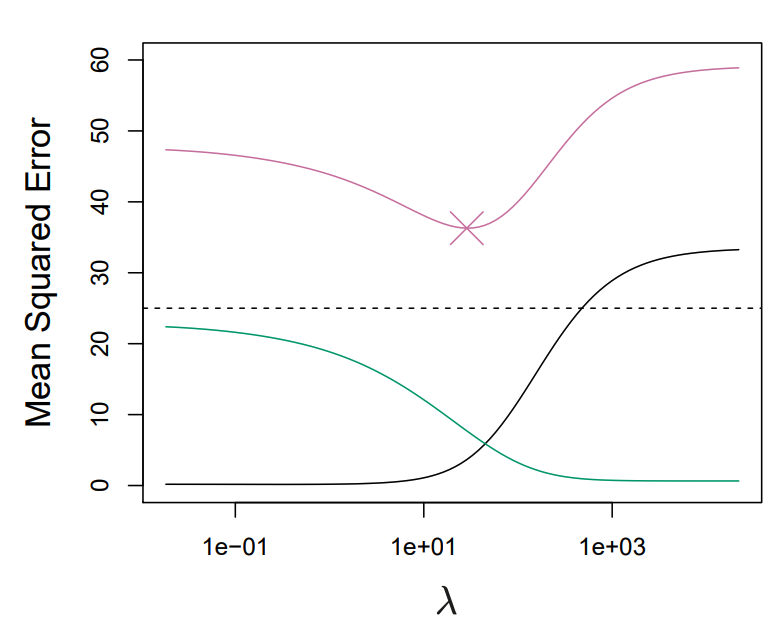
\includegraphics[width=8cm]{data/bias_variance_decomp.png}
            };
        \end{tikzpicture}
        \vfill
    \end{frame}

    \begin{frame}{Shrinkage: Outline} % Salary general model
        \centering
        \vfill
        \begin{tikzpicture}
            \node[] at (0, 0) {
                $salary \sim \beta_0 + \beta_1 * age$
            };
            \node[] at (-6, -2) {};
            \node[] at (6, 1) {};
        \end{tikzpicture}
        \vfill
    \end{frame}

    \begin{frame}{Shrinkage: Outline} % Salary actual models
        \centering
        \vfill
        \begin{tikzpicture}
            \node[] at (0, 0) {
                $salary \sim \beta_0 + \beta_1 * age$
            };

            \node[] at (3, -1) {
                $salary \sim 600000 + 0 * age$
            };

            \node[] at (-3, -1) {
                $salary \sim 300000 + 10000 * age$
            };
            \node[] at (-6, -2) {};
            \node[] at (6, 1) {};
        \end{tikzpicture}
        \vfill
    \end{frame}

    \begin{frame}{Shrinkage: Ridge regression} % MSE
        \centering
        \vfill
        \begin{tikzpicture}
            \node[inner sep=0pt] (loss) at (0, 0) {
                $= \sum\limits_{i=0}^n \left( y_i - \sum\limits_{j=0}^p \beta_j x_{ij} \right)^2$
            };
            \node[anchor=east, inner sep=0pt] at (loss.west) {
                $loss_{mse}$
            };

            \node[] at (-2.5, -2) {};
            \node[] at (3.3, 1) {};
        \end{tikzpicture}
        \vfill
    \end{frame}

    \begin{frame}{Shrinkage: Ridge regression} % Ridge loss
        \centering
        \vfill
        \begin{tikzpicture}
            \node[inner sep=0pt] (loss) at (0, 0) {
                $= \sum\limits_{i=0}^n \left( y_i - \sum\limits_{j=0}^p \beta_j x_{ij} \right)^2$
            };
            \node[anchor=west, inner sep=0pt] (ridge) at (loss.east) {
                $ + \lambda \sum\limits_{j=0}^p \beta_j^2$
            };
            \node[anchor=east, inner sep=0pt] at (loss.west) {
                $loss_{ridge}$
            };

            \node[] at (-2.5, -2) {};
            \node[] at (3.3, 1) {};
        \end{tikzpicture}
        \vfill
    \end{frame}

    \begin{frame}{Shrinkage: Ridge regression} % Ridge interpretation
        \centering
        \vfill
        \begin{tikzpicture}
            \node[inner sep=0pt] (loss) at (0, 0) {
                $= \sum\limits_{i=0}^n \left( y_i - \sum\limits_{j=0}^p \beta_j x_{ij} \right)^2$
            };
            \node[anchor=west, inner sep=0pt, draw=red] (ridge) at (loss.east) {
                $ + \lambda \sum\limits_{j=0}^p \beta_j^2$
            };
            \node[anchor=east, inner sep=0pt] at (loss.west) {
                $loss_{ridge}$
            };
            \draw[double, -Latex, red] ($ (ridge.south) - (0, 0.2) $) -- ($ (ridge.south) - (0, 0.6) $);
            \node[red] at ($ (ridge.south) - (0, 0.8) $) {
                $\lambda \to \infty \Rightarrow \beta \to 0$
            };

            \node[] at (-2.5, -2) {};
            \node[] at (3.3, 1) {};
        \end{tikzpicture}
        \vfill
    \end{frame}

    \begin{frame}{Shrinkage} % Ridge coefficients
        \centering
        \vfill
        \begin{tikzpicture}
            \node[draw=black, fill=white] {
                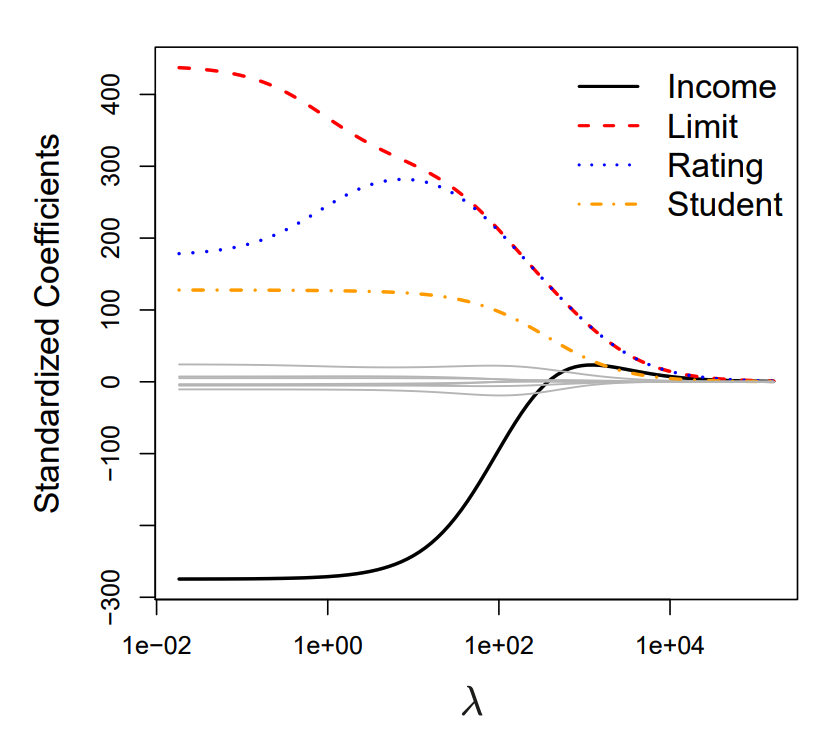
\includegraphics[width=8cm]{data/ridge_coefs.png}
            };
        \end{tikzpicture}
        \vfill
    \end{frame}

    \begin{frame}{Shrinkage: Ridge regression} % Ridge loss for scaling
        \centering
        \vfill
        \begin{tikzpicture}
            \node[inner sep=0pt] (loss) at (0, 0) {
                $= \sum\limits_{i=0}^n \left( y_i - \sum\limits_{j=0}^p \beta_j x_{ij} \right)^2$
            };
            \node[anchor=west, inner sep=0pt] (ridge) at (loss.east) {
                $ + \lambda \sum\limits_{j=0}^p \beta_j^2$
            };
            \node[anchor=east, inner sep=0pt] at (loss.west) {
                $loss_{ridge}$
            };

            \node[] at (-2.5, -2) {};
            \node[] at (3.3, 1) {};
        \end{tikzpicture}
        \vfill
    \end{frame}

    \begin{frame}{Shrinkage: Feature standardization} % Variables
        \centering
        \vfill
        \begin{tikzpicture}
            \begin{axis}[
                width=8cm,
                height=8cm,
                xlabel=Acceleration,
                ylabel=Weight
            ]
                \addplot[only marks, blue!50, opacity=0.5] table [col sep=comma, x=acceleration, y=weight] {data/Auto.csv};
            \end{axis}
        \end{tikzpicture}
        \vfill
    \end{frame}

    \def\codewidth{8cm}

    \begin{frame}[fragile]{Shrinkage: Feature standardization} % Name
        \vfill
        \centering
        \begin{tikzpicture}
            \node[] at (0, 0) {\underline{\textbf{z-score standardization}}};
            \node[] at (4.5, -7.5) {};
            \node[] at (-5, 0.5) {};
        \end{tikzpicture}
        \vfill
    \end{frame}

    \begin{frame}[fragile]{Shrinkage: Feature standardization} % Formula
        \vfill
        \centering
        \begin{tikzpicture}
            \node[] at (0, 0) {\underline{\textbf{z-score standardization}}};

            \node[] at (0, -0.7) {
                $\mathbf{x} = \frac{\mathbf{x} - \mu_x}{\sigma_x^2}$
            };
            \node[] at (4.5, -7.5) {};
            \node[] at (-5, 0.5) {};
        \end{tikzpicture}
        \vfill
    \end{frame}

    \begin{frame}[fragile]{Shrinkage: Feature standardization} % Code
        \vfill
        \centering
        \begin{tikzpicture}
            \node[] at (0, 0) {\underline{\textbf{z-score standardization}}};

            \node[] at (0, -0.7) {
                $\mathbf{x} = \frac{\mathbf{x} - \mu_x}{\sigma_x^2}$
            };

            \node[
                minimum width=\codewidth,
                text width=\codewidth,
                align=left,
                inner sep=0pt,
                outer sep=0pt,
                draw=black,
                label={[blue,
                        anchor=north east,
                        font=\ttfamily\fontsize{5}{6}\selectfont,
                        inner sep=0pt,
                        outer sep=0pt,
                        xshift=-3pt,
                        yshift=-3pt
                       ]north west:In{[}1{]}:},
            ] (pythoncode) at (0, -3) {
                \begin{lstlisting}[style=PythonStyle, linewidth=\codewidth]
for col in predictors:
    print(f'{col}: {np.mean(df[col]):.2f} ({np.std(df[col]):.2f})')

# z-score standardization
for col in predictors:
    df[col] = (df[col] - np.mean(df[col])) / np.std(df[col])

for col in predictors:
    print(f'{col} after: {np.mean(df[col]):.2f} ({np.std(df[col]):.2f})')
                \end{lstlisting}
            };
            \node[] at (4.5, -7.5) {};
            \node[] at (-5, 0.5) {};
        \end{tikzpicture}
        \vfill
    \end{frame}

    \begin{frame}[fragile]{Shrinkage: Feature standardization} % Result
        \vfill
        \centering
        \begin{tikzpicture}
            \node[] at (0, 0) {\underline{\textbf{z-score standardization}}};

            \node[] at (0, -0.7) {
                $\mathbf{x} = \frac{\mathbf{x} - \mu_x}{\sigma_x^2}$
            };

            \node[
                minimum width=\codewidth,
                text width=\codewidth,
                align=left,
                inner sep=0pt,
                outer sep=0pt,
                draw=black,
                label={[blue,
                        anchor=north east,
                        font=\ttfamily\fontsize{5}{6}\selectfont,
                        inner sep=0pt,
                        outer sep=0pt,
                        xshift=-3pt,
                        yshift=-3pt
                       ]north west:In{[}1{]}:},
            ] (pythoncode) at (0, -3) {
                \begin{lstlisting}[style=PythonStyle, linewidth=\codewidth]
for col in predictors:
    print(f'{col}: {np.mean(df[col]):.2f} ({np.std(df[col]):.2f})')

# z-score standardization
for col in predictors:
    df[col] = (df[col] - np.mean(df[col])) / np.std(df[col])

for col in predictors:
    print(f'{col} after: {np.mean(df[col]):.2f} ({np.std(df[col]):.2f})')
                \end{lstlisting}
            };

            \node[
                minimum width=\codewidth,
                text width=\codewidth,
                align=left,
                inner sep=0pt,
                label={[red,
                        anchor=north east,
                        font=\ttfamily\fontsize{5}{6}\selectfont,
                        inner sep=0pt,
                        outer sep=0pt,
                        xshift=-3pt,
                        yshift=-3.5pt,
                        text depth=0
                        ]north west:Out{[}1{]}:}
            ] (pythonout) at (0, -6) {
                \begin{lstlisting}[style=PythonOutput]
cylinders: 5.47 (1.70)
displacement: 194.41 (104.51)
horsepower: 104.47 (38.44)
weight: 2977.58 (848.32)
acceleration: 15.54 (2.76)
year: 75.98 (3.68)
cylinders after: -0.00 (1.00)
displacement after: -0.00 (1.00)
horsepower after: -0.00 (1.00)
weight after: -0.00 (1.00)
acceleration after: 0.00 (1.00)
year after: -0.00 (1.00)
                \end{lstlisting}
            };
            \node[] at (4.5, -7.5) {};
            \node[] at (-5, 0.5) {};
        \end{tikzpicture}
        \vfill
    \end{frame}

    \begin{frame}{Shrinkage: Ridge regression}
        \centering
        \vfill
        \href{http://localhost:8888/notebooks/notebooks/Live\%20coding.ipynb}{http://localhost:8888/notebooks/notebooks/Live\%20coding.ipynb}
        \vfill
    \end{frame}

    \begin{frame}{Shrinkage: Ridge regression}
        \centering
        \vfill
        \begin{tikzpicture}
            \node[inner sep=0pt] (loss) at (0, 0) {
                $= \sum\limits_{i=0}^n \left( y_i - \sum\limits_{j=0}^p \beta_j x_{ij} \right)^2$
            };
            \node[anchor=west, inner sep=0pt] (ridge) at (loss.east) {
                $ + \lambda \sum\limits_{j=0}^p \beta_j^2$
            };
            \node[anchor=east, inner sep=0pt] at (loss.west) {
                $loss_{ridge}$
            };

            \node[] at (0, -1.5) {
                Regularization through shrinking the model covariates towards zero.
            };

            \node[] at (-4.4, -4) {};
            \node[] at (5.2, 3) {};
        \end{tikzpicture}
        \vfill
    \end{frame}

    \begin{frame}{Shrinkage: LASSO} % Formula
        \centering
        \vfill
        \begin{tikzpicture}
            \node[inner sep=0pt] (loss) at (0, 0) {
                $= \sum\limits_{i=0}^n \left( y_i - \sum\limits_{j=0}^p \beta_j x_{ij} \right)^2$
            };
            \node[anchor=west, inner sep=0pt] (ridge) at (loss.east) {
                $ + \lambda \sum\limits_{j=0}^p \beta_j^2$
            };
            \node[anchor=east, inner sep=0pt] at (loss.west) {
                $loss_{ridge}$
            };


            \node[inner sep=0pt] (lassomse) at (0, -2) {
                $= \sum\limits_{i=0}^n \left( y_i - \sum\limits_{j=0}^p \beta_j x_{ij} \right)^2$
            };
            \node[anchor=west, inner sep=0pt] (lasso) at (lassomse.east) {
                $ + \lambda \sum\limits_{j=0}^p |\beta_j|$
            };
            \node[anchor=east, inner sep=0pt] at (lassomse.west) {
                $loss_{lasso}$
            };

            \node[] at (-4.4, -4) {};
            \node[] at (5.2, 3) {};
        \end{tikzpicture}
        \vfill
    \end{frame}

    \begin{frame}{Shrinkage: LASSO} % Ridge coefficients
        \vfill
        \centering
        \begin{tikzpicture}
            \node[fill=white, draw=black, label=Ridge] at (0, 0) {
                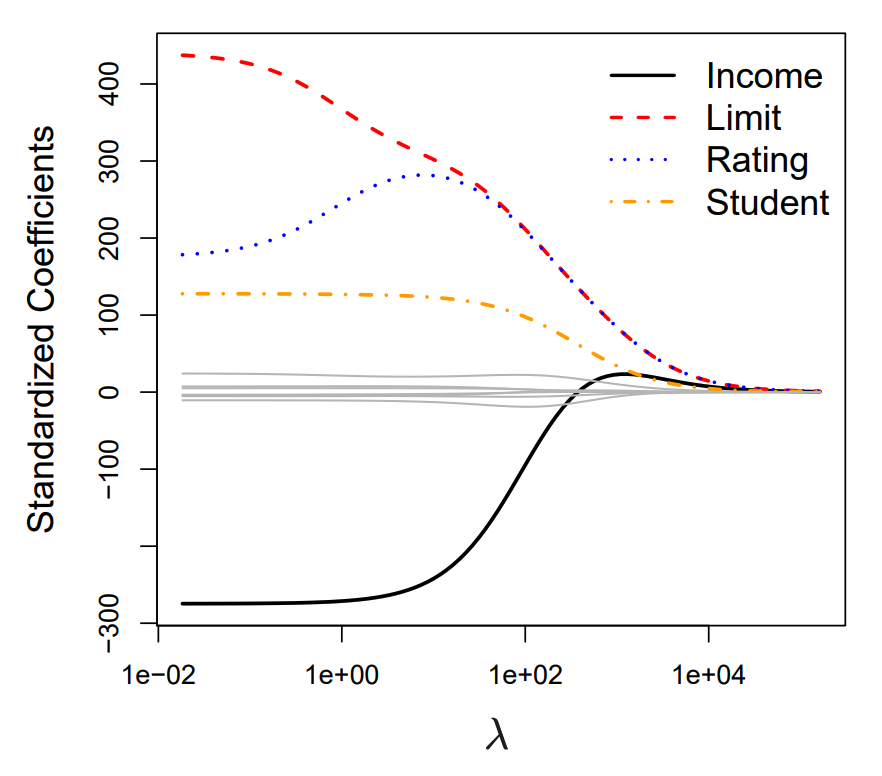
\includegraphics[width=4cm]{data/ridge.png}
            };

            \node[] at (-2.5, -2.5) {};
            \node[] at (7.5, 2.5) {};
        \end{tikzpicture}
        \vfill
    \end{frame}

    \begin{frame}{Shrinkage: LASSO} % Lasso coefficients
        \vfill
        \centering
        \begin{tikzpicture}
            \node[fill=white, draw=black, label=Ridge] at (0, 0) {
                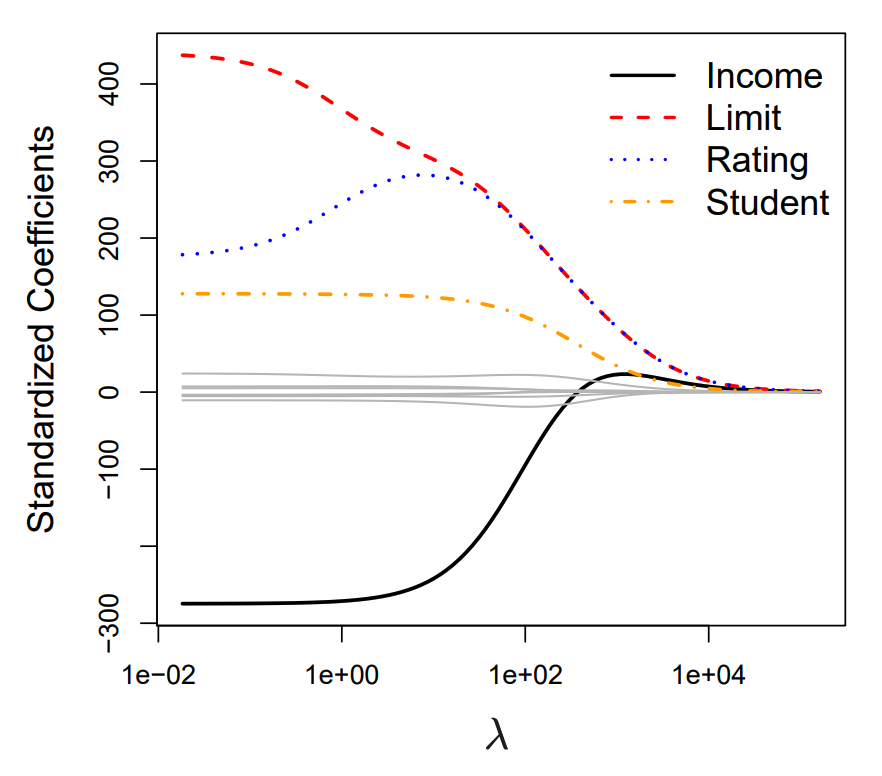
\includegraphics[width=4cm]{data/ridge.png}
            };
            \node[fill=white, draw=black, label=LASSO] at (5, 0) {
                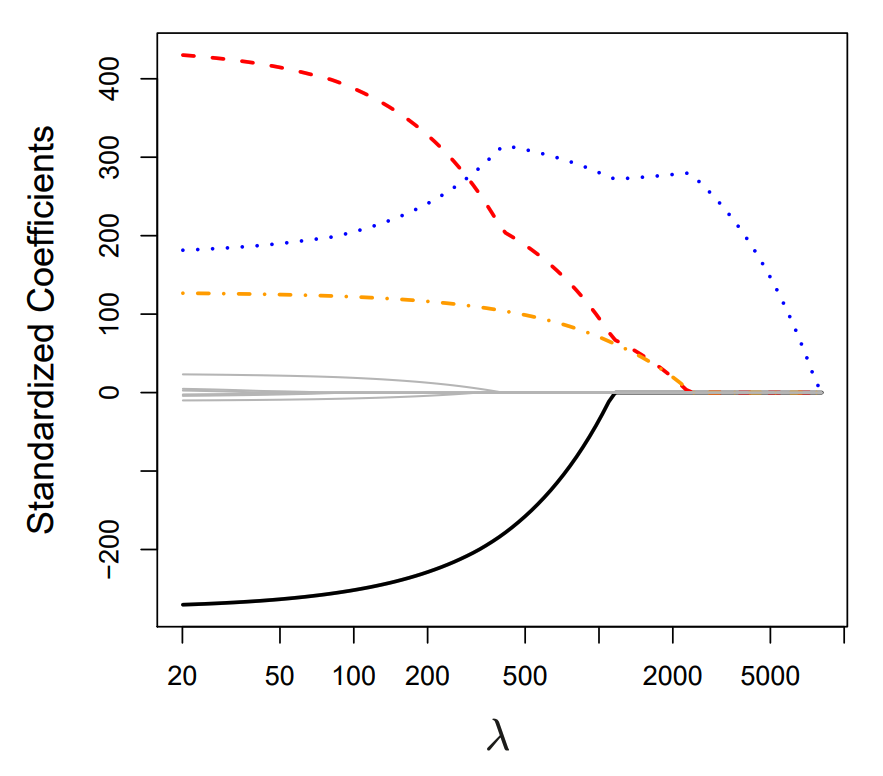
\includegraphics[width=4cm]{data/lasso.png}
            };

            \node[] at (-2.5, -2.5) {};
            \node[] at (7.5, 2.5) {};
        \end{tikzpicture}
        \vfill
    \end{frame}

    \begin{frame}[t]{Shrinkage: LASSO} % Table of coefficients
        \centering
        \vspace{2cm}
        \begin{tabular}{|c|c|c|}
            \hline
            \textbf{Predictor}&\textbf{Ridge}&\textbf{LASSO}\\
            \hline
            Intercept&23.44&23.44\\
            \hline
            Weight&-5.59&-4.78\\
            \hline
            Year&2.75&2.00\\
            \hline
            Horsepower&-0.07&-0.09\\
            \hline
            Cylinders&-0.54&0\\
            \hline
            Acceleration&0.19&0\\
            \hline
            Displacement&0.66&0\\
            \hline
        \end{tabular}
    \end{frame}


    \begin{frame}[t]{Shrinkage: LASSO} % Table of coefficients
        \centering
        \vspace{2cm}
        \begin{tabular}{|c|c|c|}
            \hline
            \textbf{Predictor}&\textbf{Ridge}&\textbf{LASSO}\\
            \hline
            Intercept&23.44&23.44\\
            \hline
            Weight&-5.59&-4.78\\
            \hline
            Year&2.75&2.00\\
            \hline
            Horsepower&-0.07&-0.09\\
            \hline
            Cylinders&-0.54&0\\
            \hline
            Acceleration&0.19&0\\
            \hline
            Displacement&0.66&0\\
            \hline
        \end{tabular}\\
        \vspace{1cm}
        \textcolor{red}{A coefficient of 0 does not mean the predictor has no predictive value for the outcome!}
    \end{frame}

    \begin{frame}{Shrinkage: LASSO} % Lasso intuition
        \centering
        \vfill
        \begin{tikzpicture}
            \node[fill=white, draw=black] at (0, 0) {
                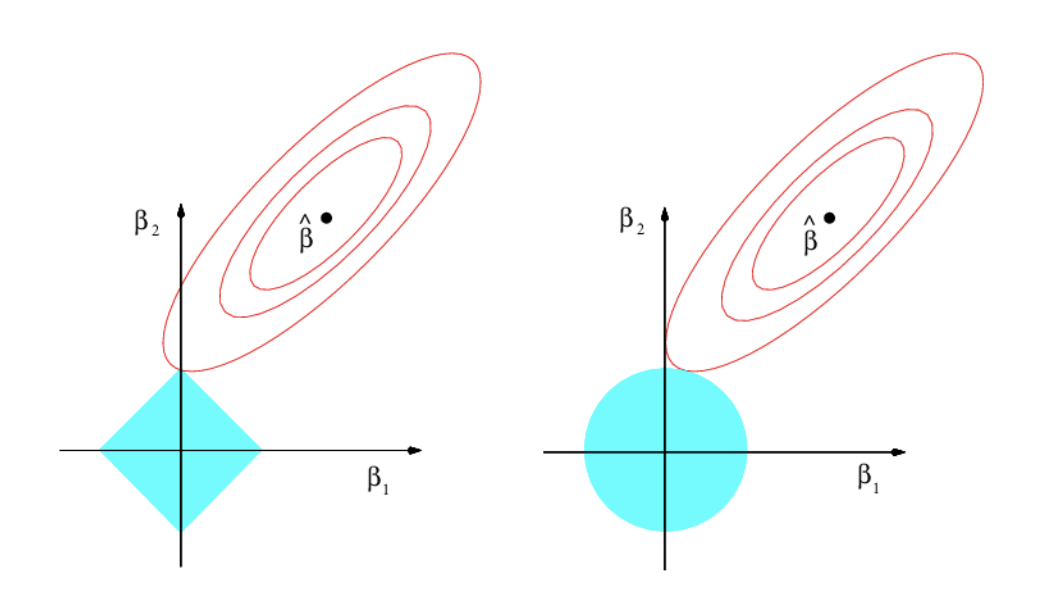
\includegraphics[width=8cm]{data/lasso_intuition.png}
            };
        \end{tikzpicture}\\
        \vspace{0.5cm}
        Whiteboard! \emoji{partying-face}
        \vfill
    \end{frame}

    \begin{frame}{Shrinkage: LASSO} % Lasso vs Ridge effect
        \vfill
        \centering
        \begin{tikzpicture}
            \node[fill=white, draw=black] at (0, 0) {
                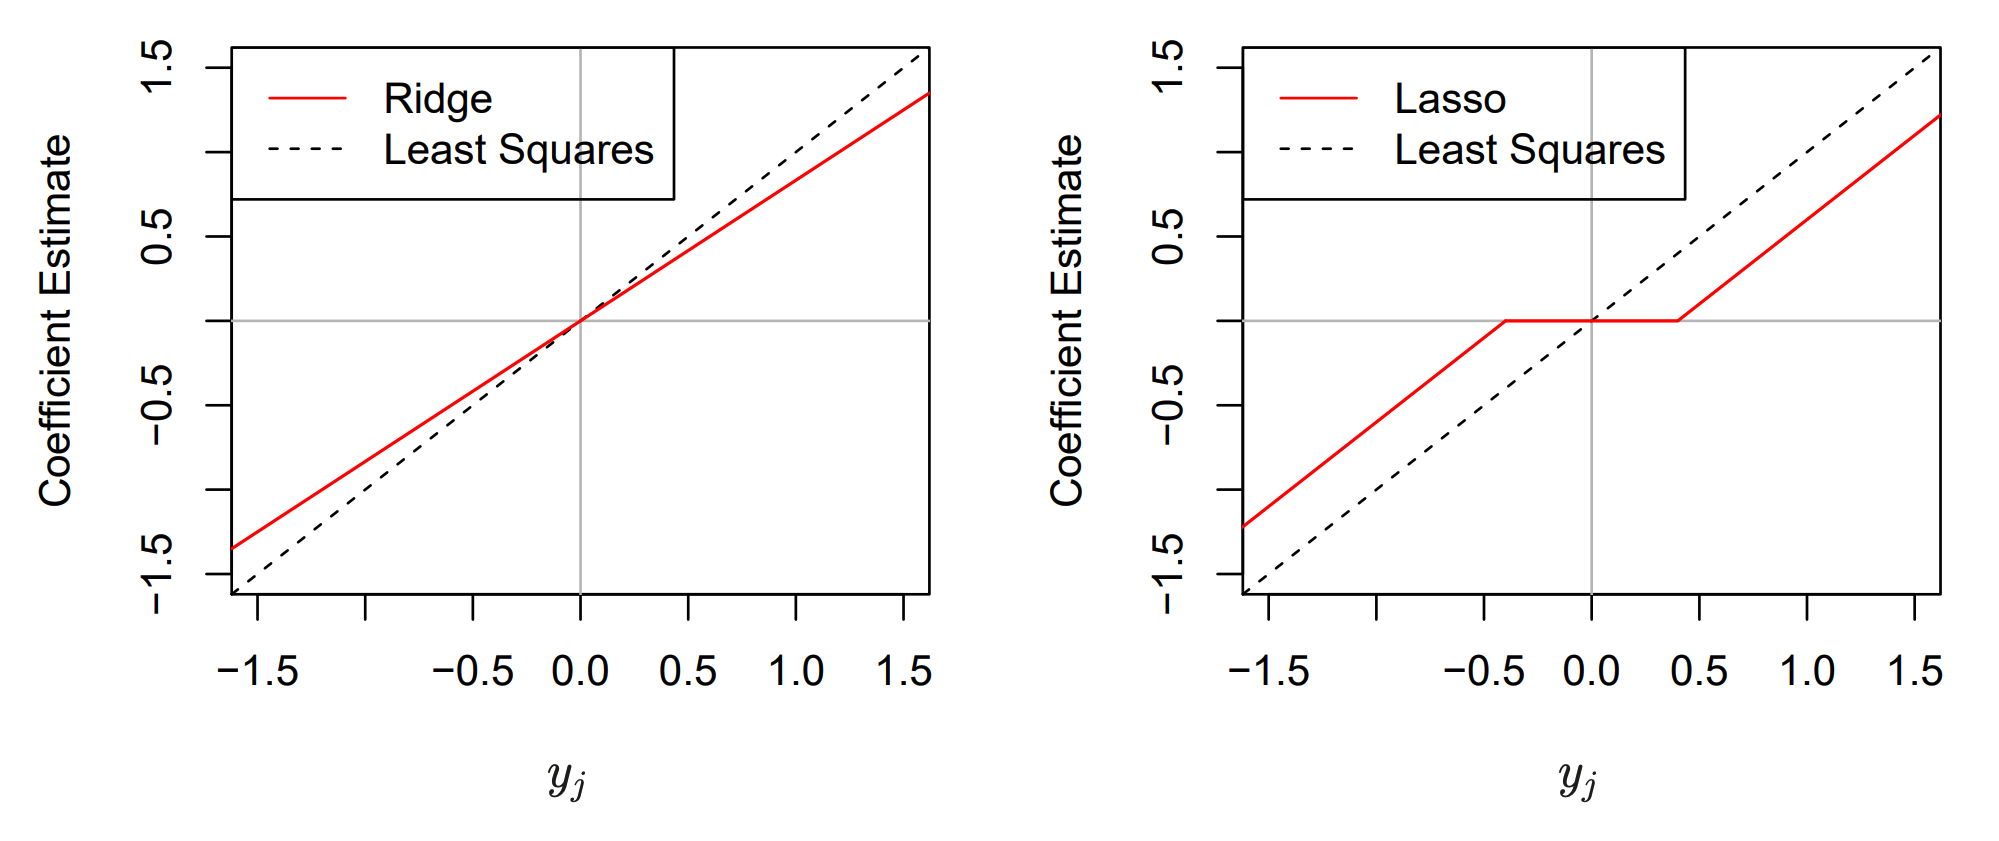
\includegraphics[width=10cm]{data/ridge_vs_lasso.png}
            };
        \end{tikzpicture}
        \vfill
    \end{frame}

    \begin{frame}{Shrinkage: LASSO} % Lasso vs ridge priors
        \vfill
        \centering
        \begin{tikzpicture}
            \node[fill=white, draw=black] at (0, 0) {
                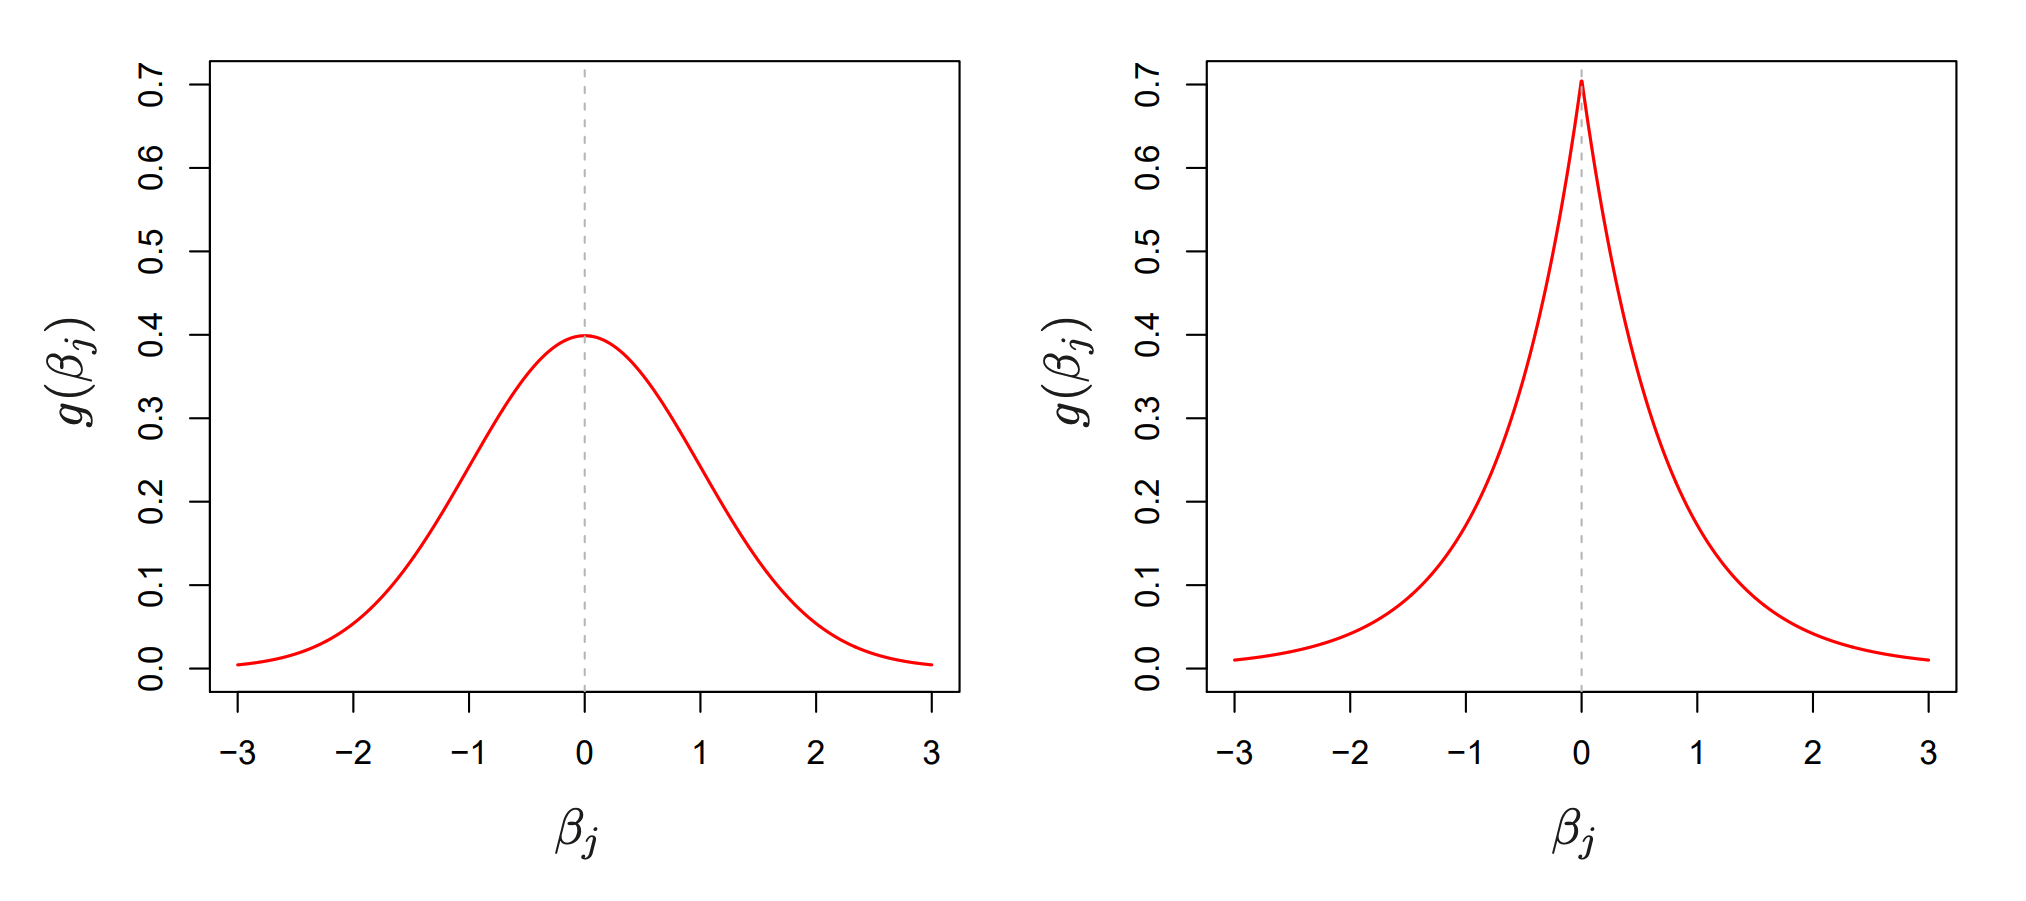
\includegraphics[width=9.5cm]{data/shrinkage_priors.png}
            };
        \end{tikzpicture}
        \vfill
    \end{frame}

    \begin{frame}{Shrinkage: Summary} % MSE
        \centering
        \vfill
        \begin{tikzpicture}
            \node[inner sep=0pt] (mse) at (0, 2.2) {
                $= \sum\limits_{i=0}^n \left( y_i - \sum\limits_{j=0}^p \beta_j x_{ij} \right)^2$
            };
            \node[anchor=east, inner sep=0pt] at (mse.west) {
                $loss_{mse}$
            };

            \node[anchor=west, align=left] at ($ (mse.west) + (4.7, 0) $) {Fits the \textbf{best} model\\to the data.};

            \node[] at (-3, -4) {};
            \node[] at (6.8, 3) {};

            \draw[black] (3.2, 3) -- (3.2, -3.9);
        \end{tikzpicture}
        \vfill
    \end{frame}

    \begin{frame}{Shrinkage: Summary} % Ridge
        \centering
        \vfill
        \begin{tikzpicture}
            \node[inner sep=0pt] (mse) at (0, 2.2) {
                $= \sum\limits_{i=0}^n \left( y_i - \sum\limits_{j=0}^p \beta_j x_{ij} \right)^2$
            };
            \node[anchor=east, inner sep=0pt] at (mse.west) {
                $loss_{mse}$
            };


            \node[inner sep=0pt] (ridgemse) at (0, 0) {
                $= \sum\limits_{i=0}^n \left( y_i - \sum\limits_{j=0}^p \beta_j x_{ij} \right)^2$
            };
            \node[anchor=west, inner sep=0pt] (lasso) at (ridgemse.east) {
                $ + \lambda \sum\limits_{j=0}^p \beta_j^2$
            };
            \node[anchor=east, inner sep=0pt] at (ridgemse.west) {
                $loss_{ridge}$
            };


            \node[anchor=west, align=left] at ($ (mse.west) + (4.7, 0) $) {Fits the \textbf{best} model\\to the data.};
            \node[anchor=west, align=left] at ($ (ridgemse.west) + (4.7, 0) $) {Fits the \textbf{best} model\\to the data while\\\textbf{shrinking} coefficients\\towards zero.};

            \node[] at (-3, -4) {};
            \node[] at (6.8, 3) {};

            \draw[black] (3.2, 3) -- (3.2, -3.9);
        \end{tikzpicture}
        \vfill
    \end{frame}

    \begin{frame}{Shrinkage: Summary} % LASSO
        \centering
        \vfill
        \begin{tikzpicture}
            \node[inner sep=0pt] (mse) at (0, 2.2) {
                $= \sum\limits_{i=0}^n \left( y_i - \sum\limits_{j=0}^p \beta_j x_{ij} \right)^2$
            };
            \node[anchor=east, inner sep=0pt] at (mse.west) {
                $loss_{mse}$
            };


            \node[inner sep=0pt] (ridgemse) at (0, 0) {
                $= \sum\limits_{i=0}^n \left( y_i - \sum\limits_{j=0}^p \beta_j x_{ij} \right)^2$
            };
            \node[anchor=west, inner sep=0pt] (lasso) at (ridgemse.east) {
                $ + \lambda \sum\limits_{j=0}^p \beta_j^2$
            };
            \node[anchor=east, inner sep=0pt] at (ridgemse.west) {
                $loss_{ridge}$
            };


            \node[inner sep=0pt] (lassomse) at (0, -2.2) {
                $= \sum\limits_{i=0}^n \left( y_i - \sum\limits_{j=0}^p \beta_j x_{ij} \right)^2$
            };
            \node[anchor=west, inner sep=0pt] (lasso) at (lassomse.east) {
                $ + \lambda \sum\limits_{j=0}^p |\beta_j|$
            };
            \node[anchor=east, inner sep=0pt] at (lassomse.west) {
                $loss_{lasso}$
            };

            \node[anchor=west, align=left] at ($ (mse.west) + (4.7, 0) $) {Fits the \textbf{best} model\\to the data.};
            \node[anchor=west, align=left] at ($ (ridgemse.west) + (4.7, 0) $) {Fits the \textbf{best} model\\to the data while\\\textbf{shrinking} coefficients\\towards zero.};
            \node[anchor=west, align=left] at ($ (lassomse.west) + (4.7, 0) $) {Fits the \textbf{best} model\\to the data while\\\textbf{shrinking} coefficients\\towards zero such\\that some variables\\are effectively \textbf{removed}.};

            \node[] at (-3, -4) {};
            \node[] at (6.8, 3) {};

            \draw[black] (3.2, 3) -- (3.2, -3.9);
        \end{tikzpicture}
        \vfill
    \end{frame}

    % \section{Dimensionality reduction}

    % \begin{frame}{Dimensionality reduction: Motivation}
    %     \centering
    %     Although we have $p$ predictors, there are actually $q<p$ dimensions of variability in our data, and using $q$ predictors instead of $p$ predcitors is going to reduce model complexity.
    % \end{frame}
\end{document}
